% Created 2018-06-21 Thu 12:30
\documentclass[8pt]{beamer}
\usepackage[sc,osf]{mathpazo}   % With old-style figures and real smallcaps.
\linespread{1.025}              % Palatino leads a little more leading
% Euler for math and numbers
\usepackage[euler-digits,small]{eulervm}
%\documentclass[10pt]{llncs}
%\usepackage{llncsdoc}
\usepackage{minted}
\usepackage[utf8]{inputenc}
\usepackage[T1]{fontenc}
\usepackage{fixltx2e}
\usepackage{graphicx}
\usepackage{longtable}
\usepackage{float}
\usepackage{wrapfig}
\usepackage{rotating}
\usepackage[normalem]{ulem}
\usepackage{amsmath}
\usepackage{textcomp}
\usepackage{marvosym}
\usepackage{wasysym}
\usepackage{amssymb}
\usepackage{hyperref}
\usepackage{polynom}
\renewcommand{\mod}[1]{\left( \texttt{mod}~#1 \right)}
\newcommand{\N}{\mathbb N}
\newcommand{\Z}{\mathbb Z}
\newcommand{\Q}{\mathbb Q}
\newcommand{\C}{\mathbb C}
\newcommand{\degree}{\texttt{degree}}
\newcommand{\node}{\texttt{node}}
\newcommand{\class}{\texttt{class}}
\newcommand{\egg}{\texttt{egg} }
\tolerance=1000
%\usetheme{Antibes}
\addtobeamertemplate{navigation symbols}{}{%
    \usebeamerfont{footline}%
    \usebeamercolor[fg]{footline}%
    \hspace{1em}%
    \insertframenumber/\inserttotalframenumber
}


\author{Siddharth Bhat}
\date{Monday, Jan 18 2021}
\title{\egg: Fast and extensible equality saturation}
\hypersetup{
  pdfkeywords={},
  pdfsubject={},
  pdfcreator={Emacs 24.5.1 (Org mode 8.2.10)}}
\begin{document}

\titlegraphic{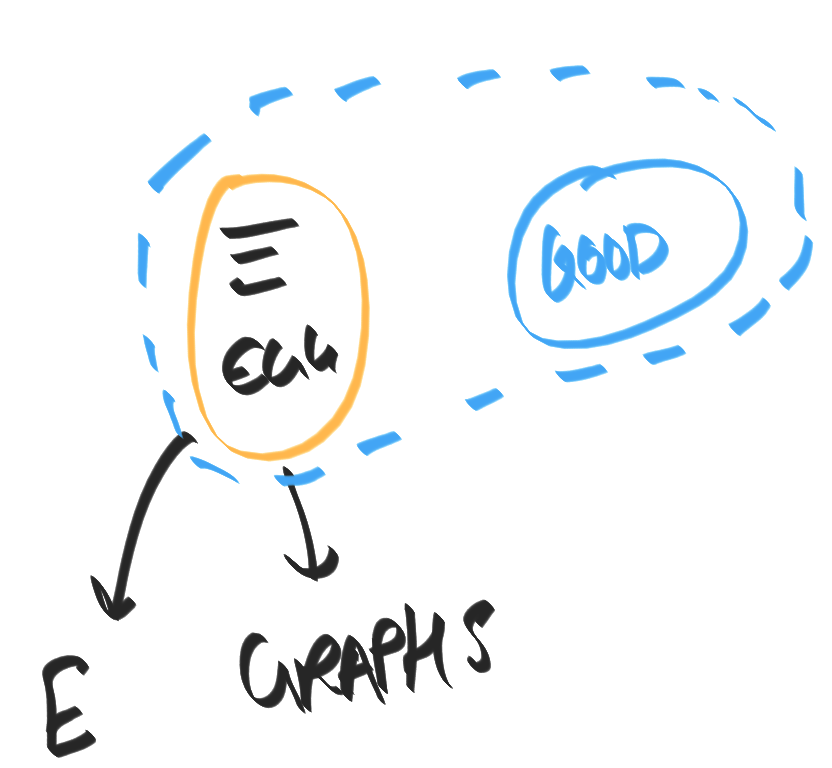
\includegraphics[width=.3\textwidth,height=.3\textheight]{./e-graphs-good.png}}


\maketitle

\begin{frame}[fragile]{\egg: Fast and extensible equality saturation}
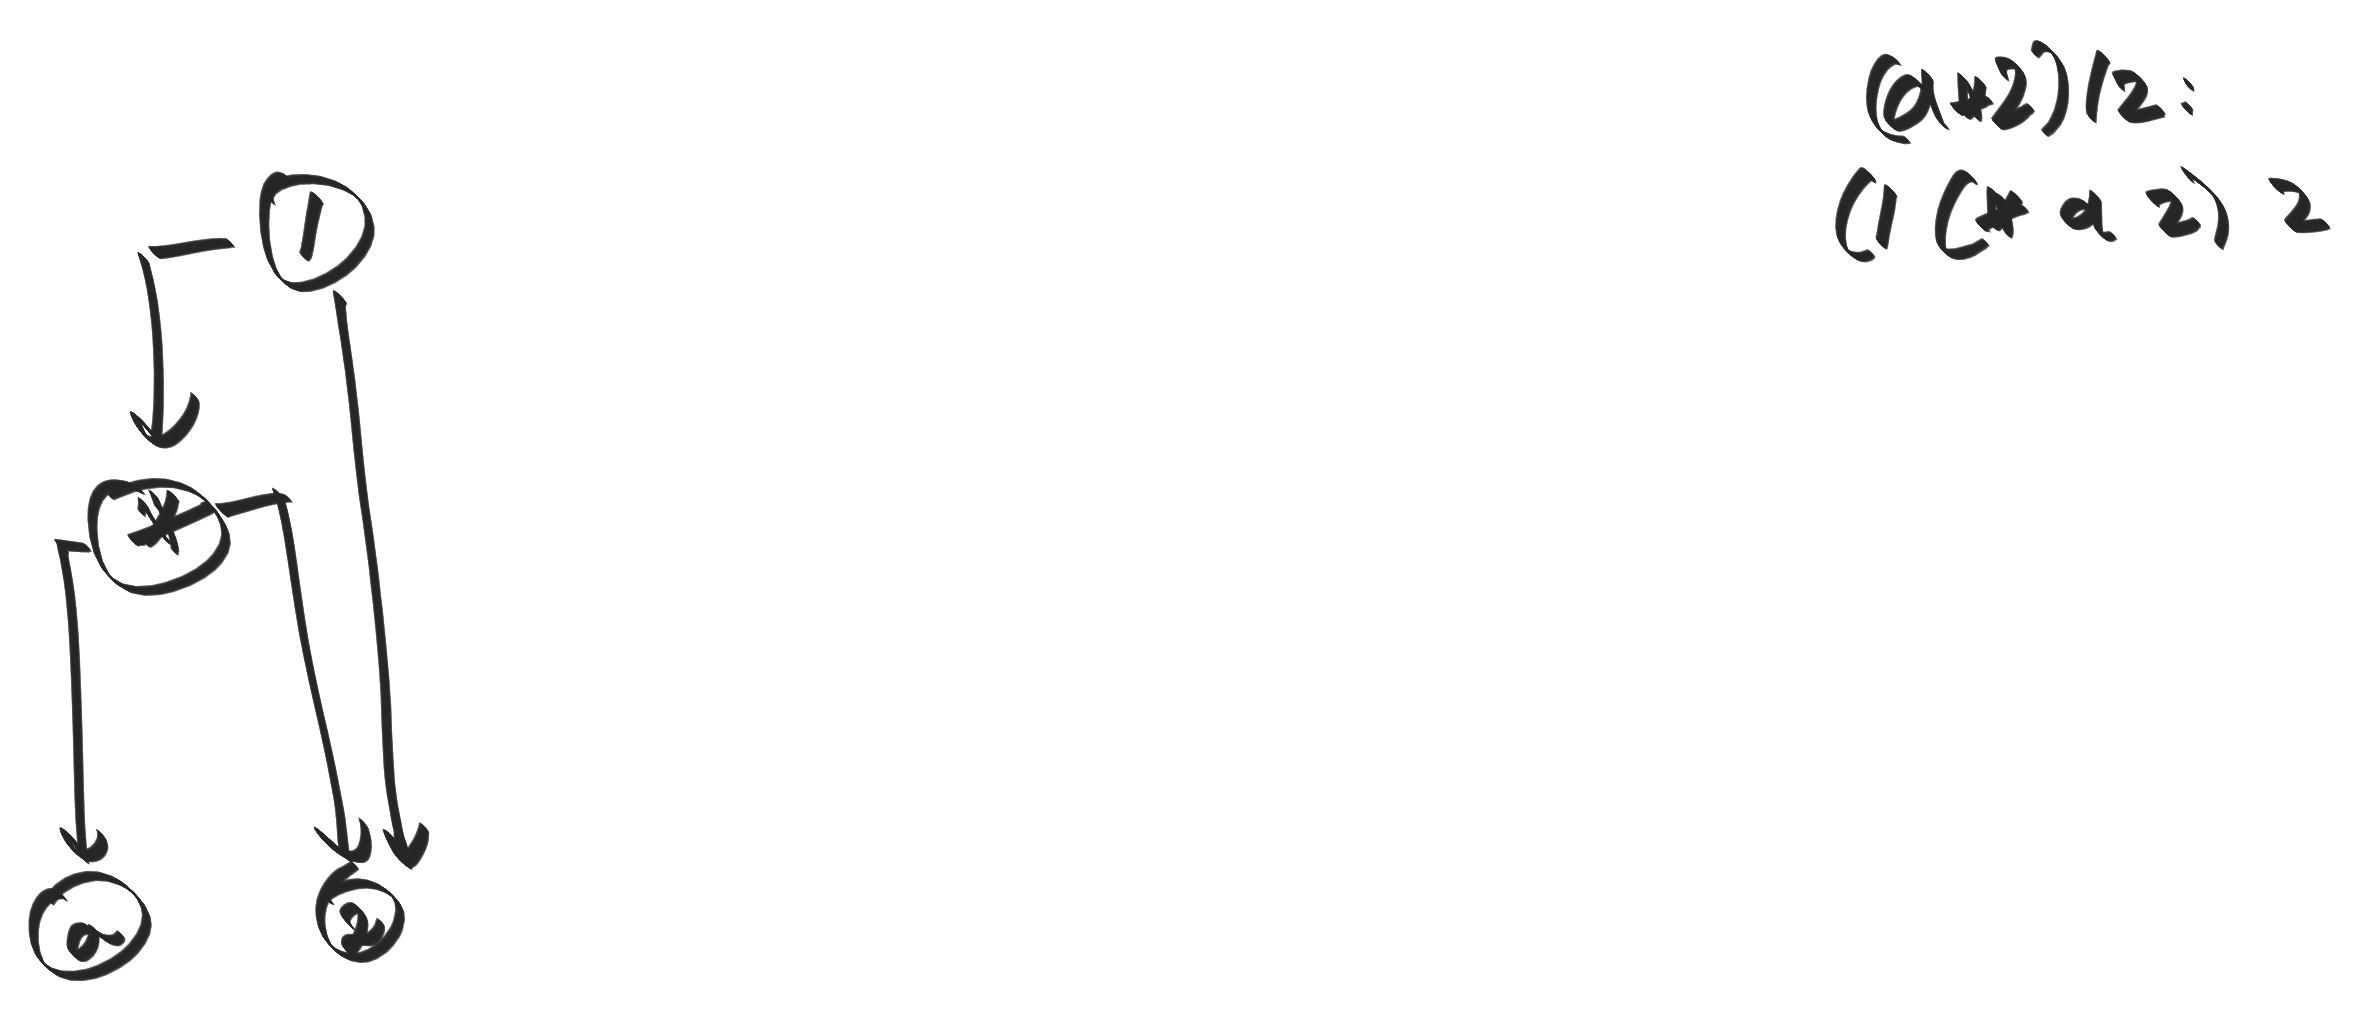
\includegraphics[width=\textwidth]{./eg-1-1.png}
\end{frame}

\begin{frame}[fragile]{\egg: Fast and extensible equality saturation (2)}
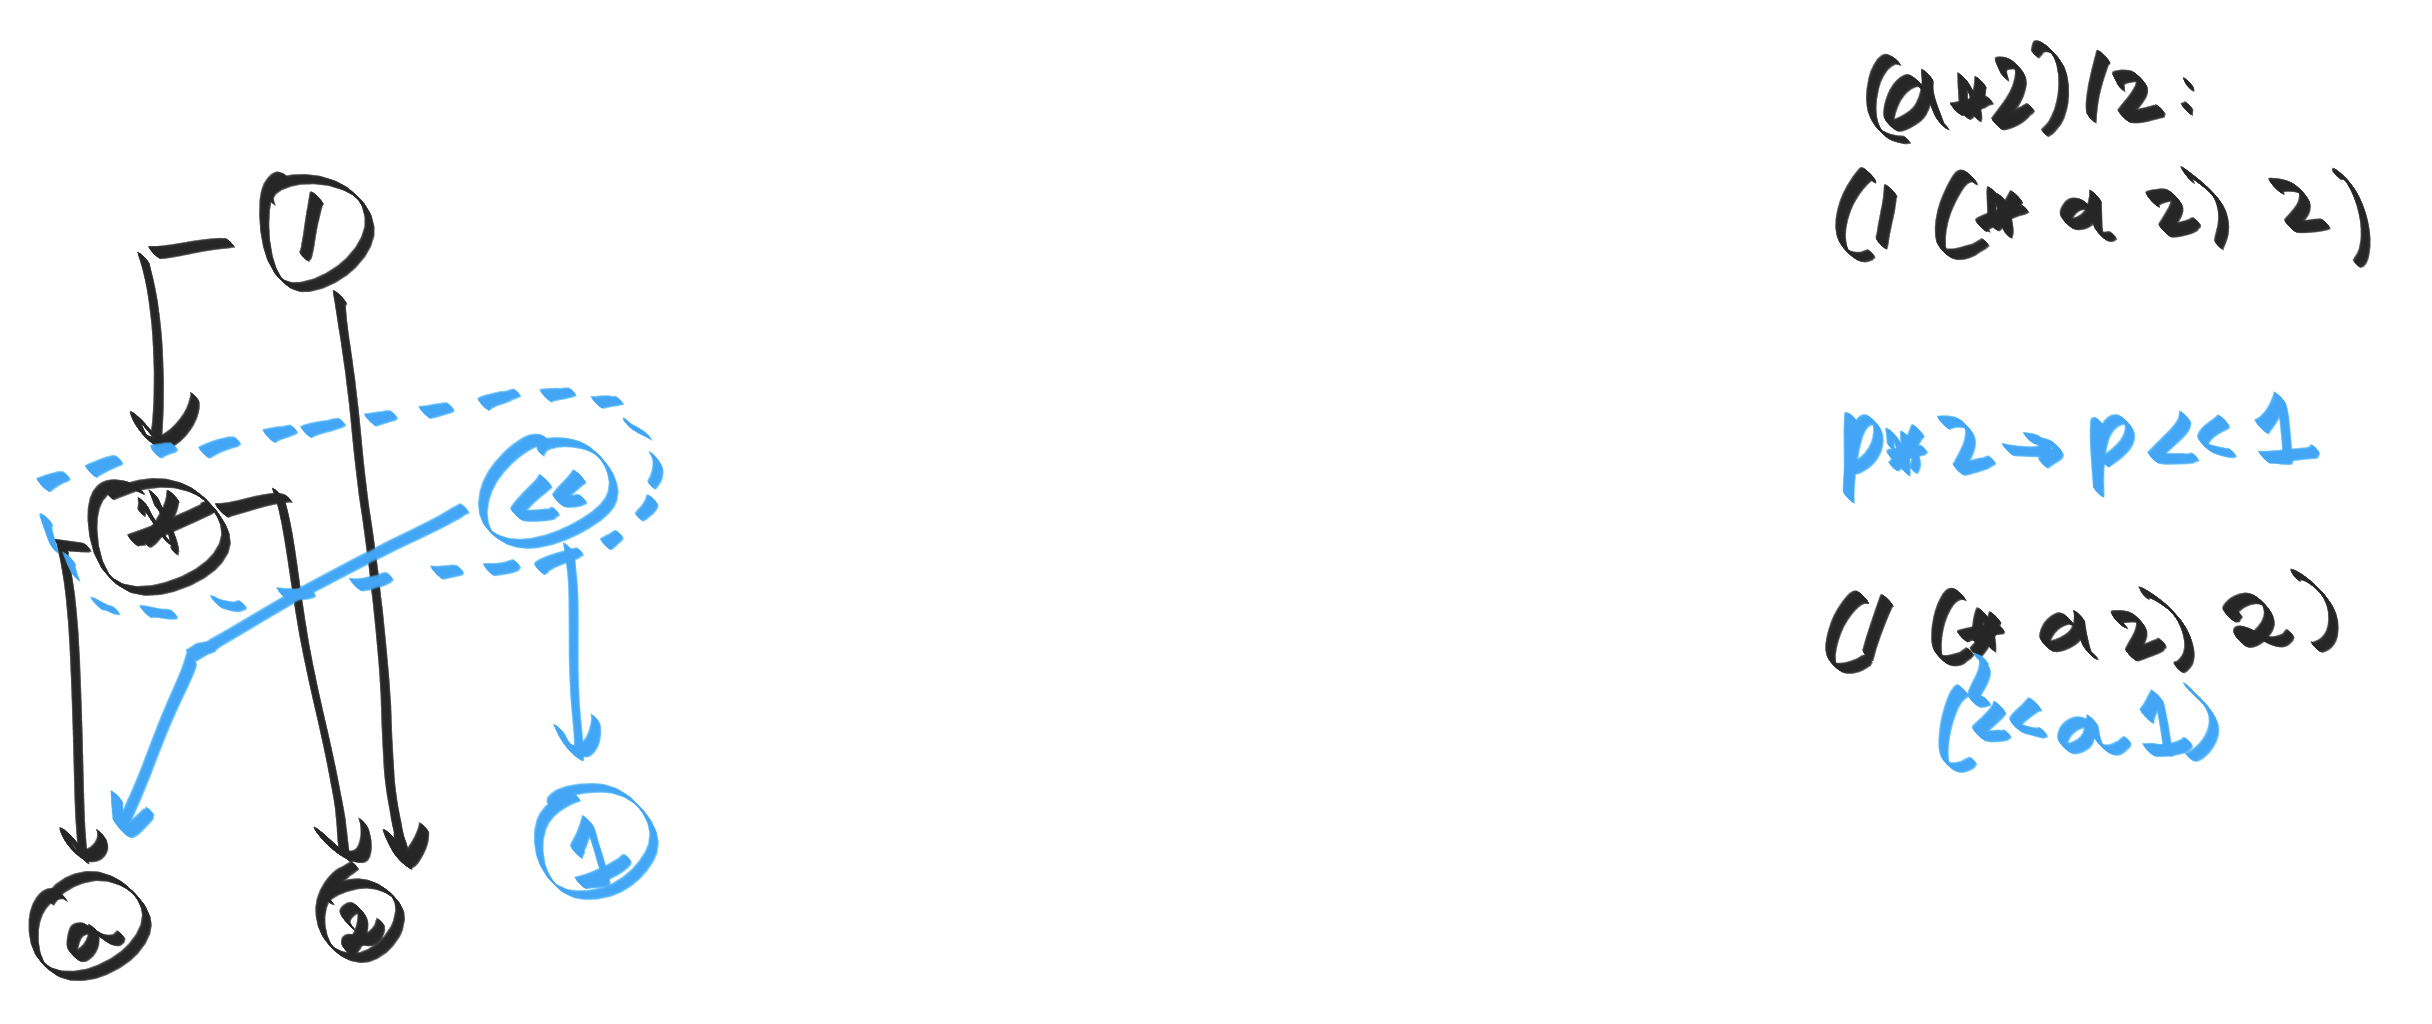
\includegraphics[width=\textwidth]{./eg-1-2.png}
\end{frame}


\begin{frame}[fragile]{\egg: Fast and extensible equality saturation (3)}
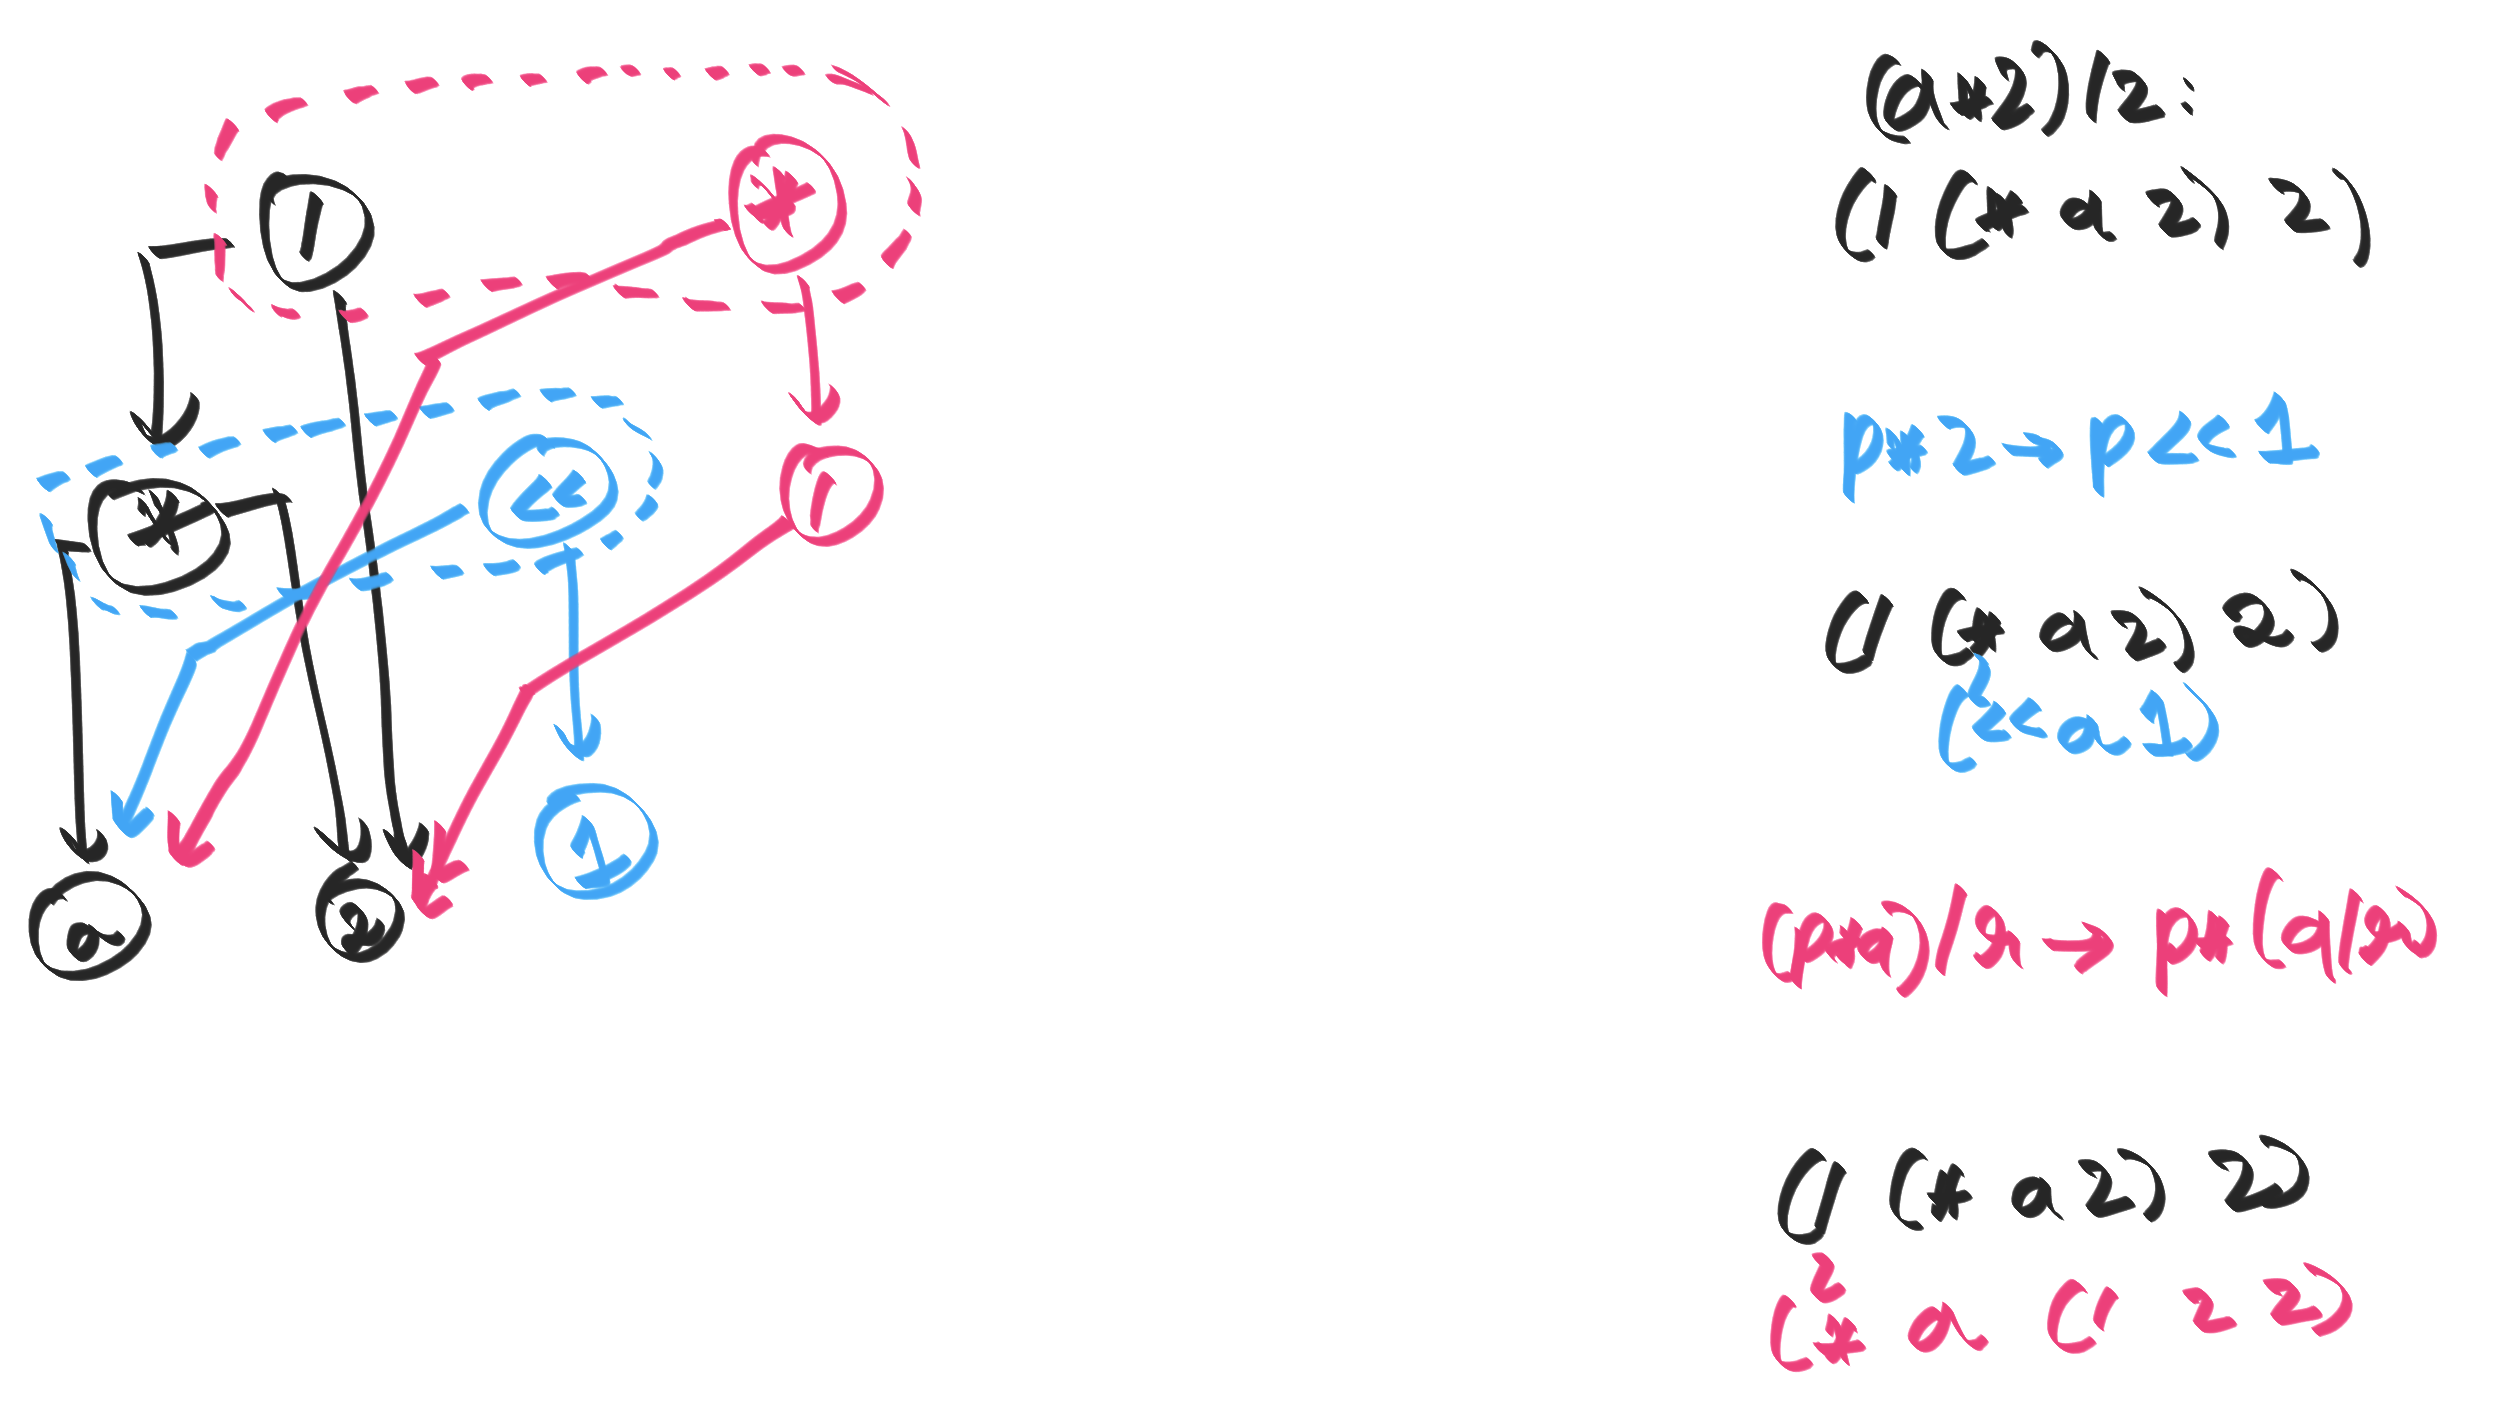
\includegraphics[width=\textwidth]{./eg-1-3.png}
\end{frame}

\begin{frame}[fragile]{\egg: Fast and extensible equality saturation (4)}
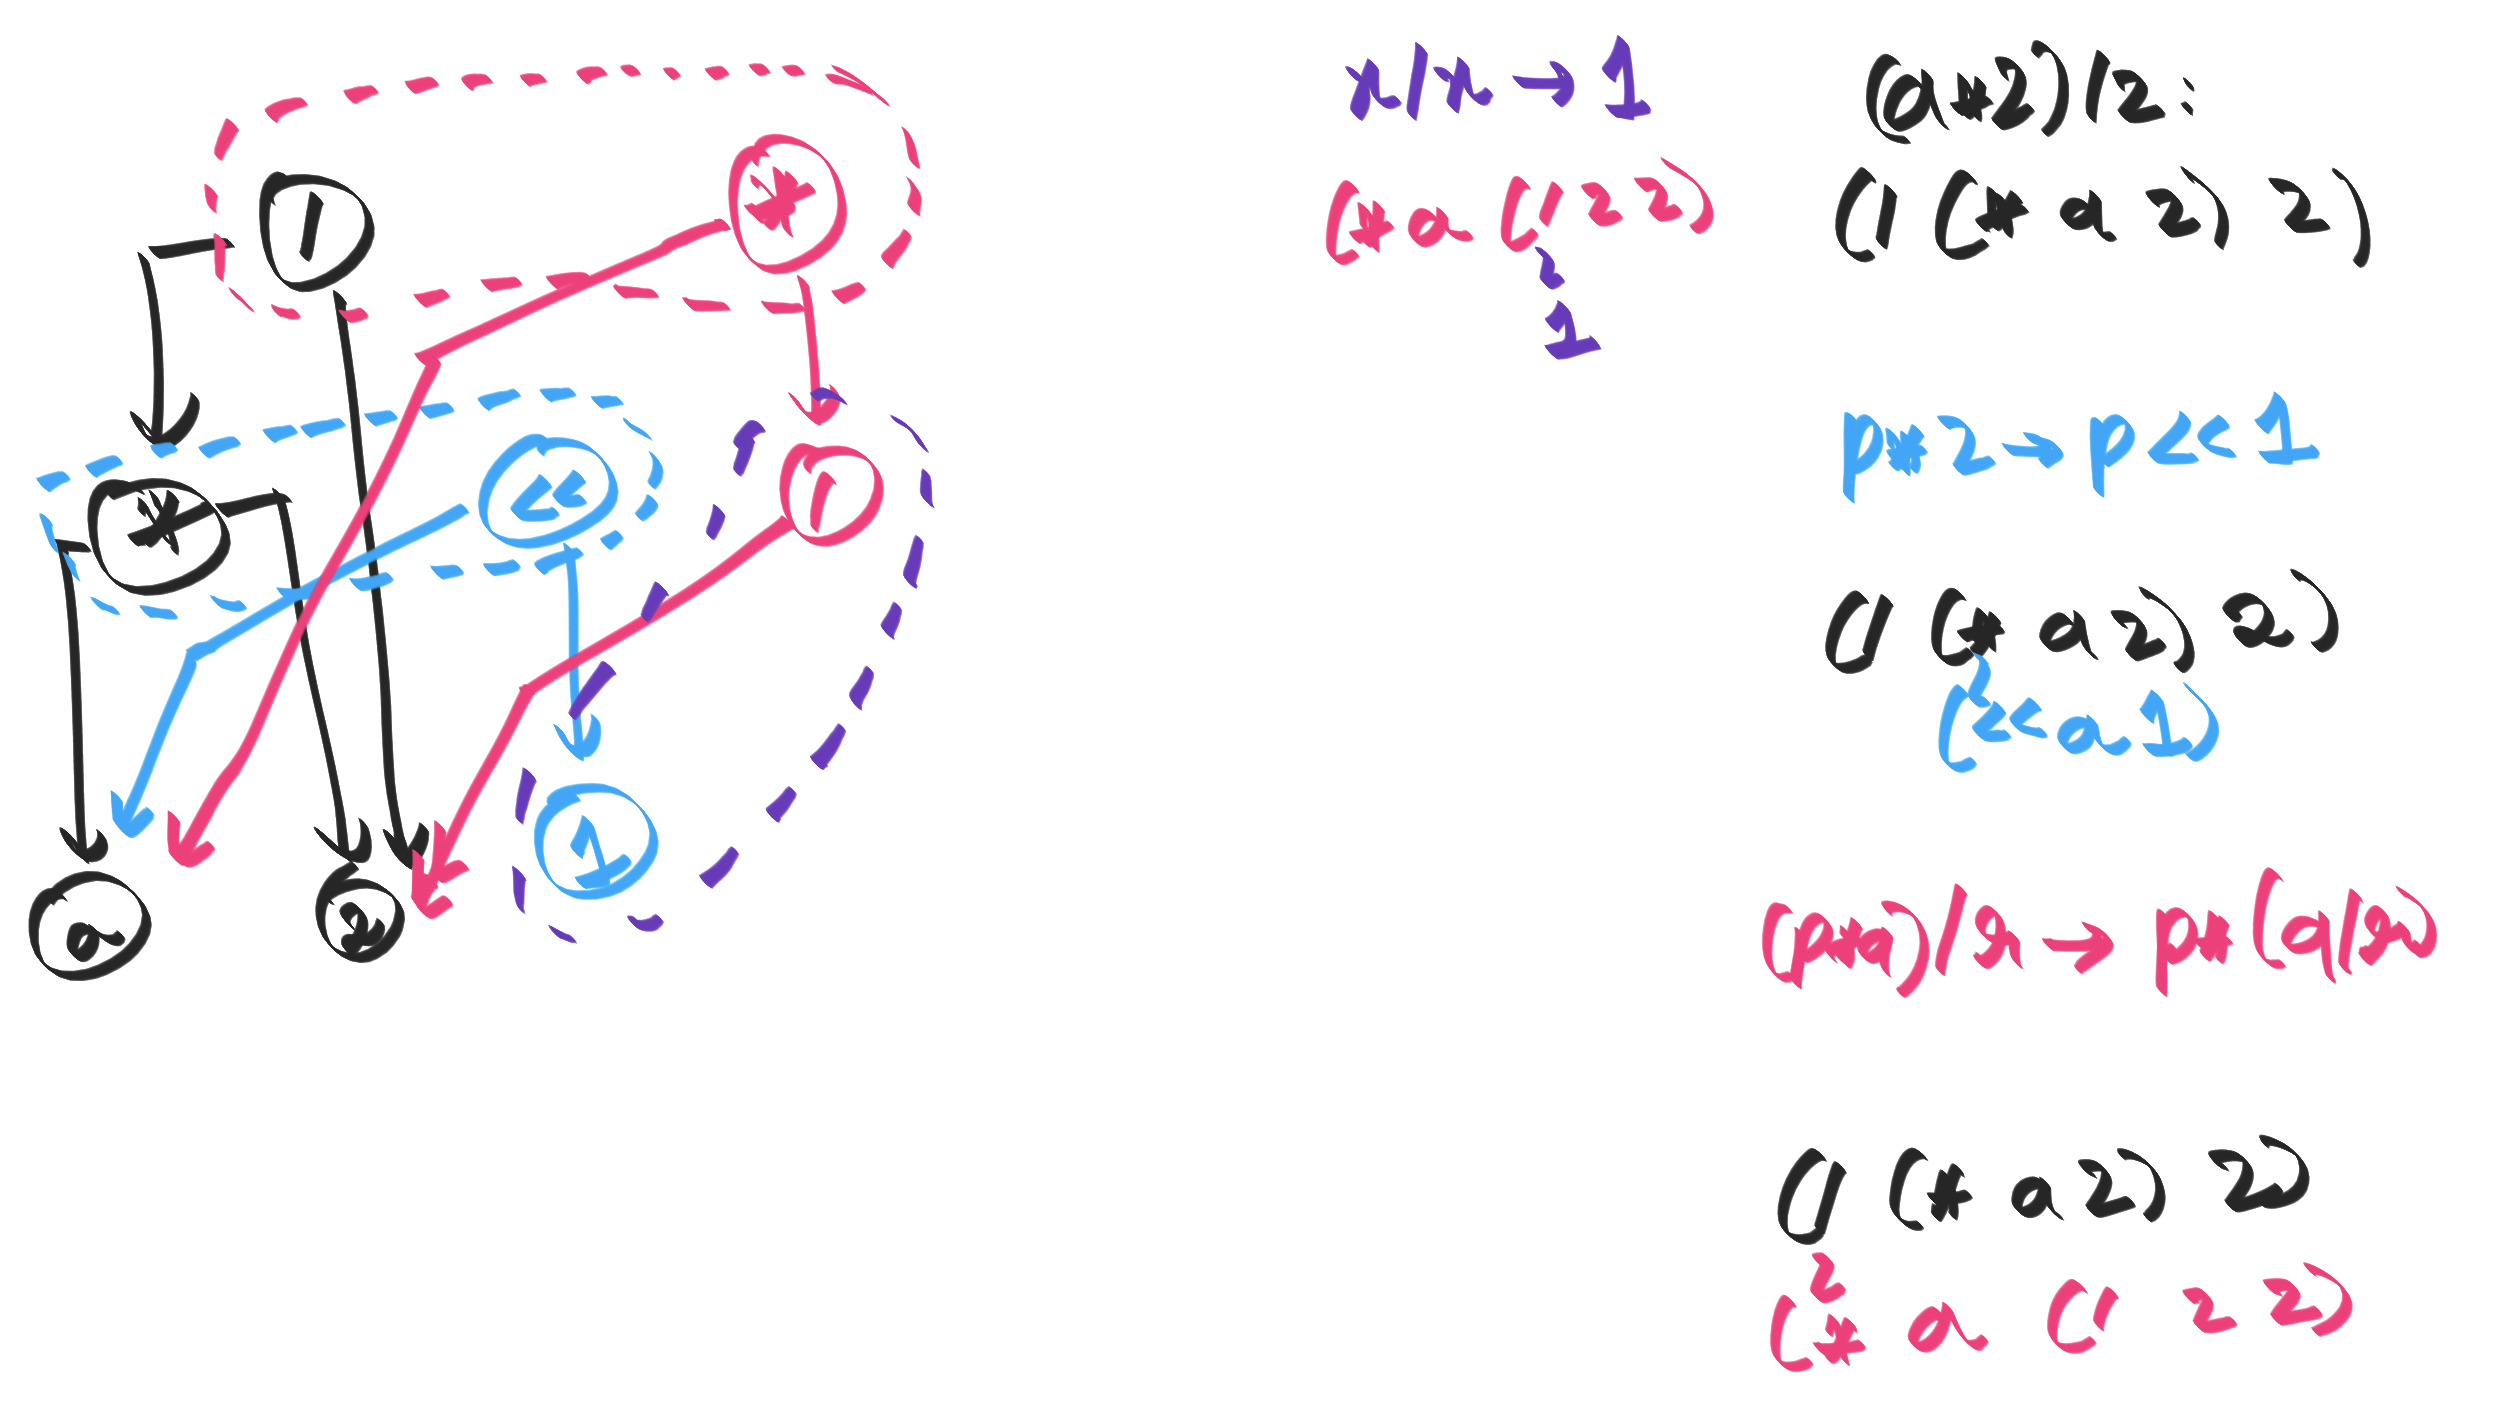
\includegraphics[width=\textwidth]{./eg-1-4.png}
\end{frame}


\begin{frame}[fragile]{\egg: Fast and extensible equality saturation (5)}
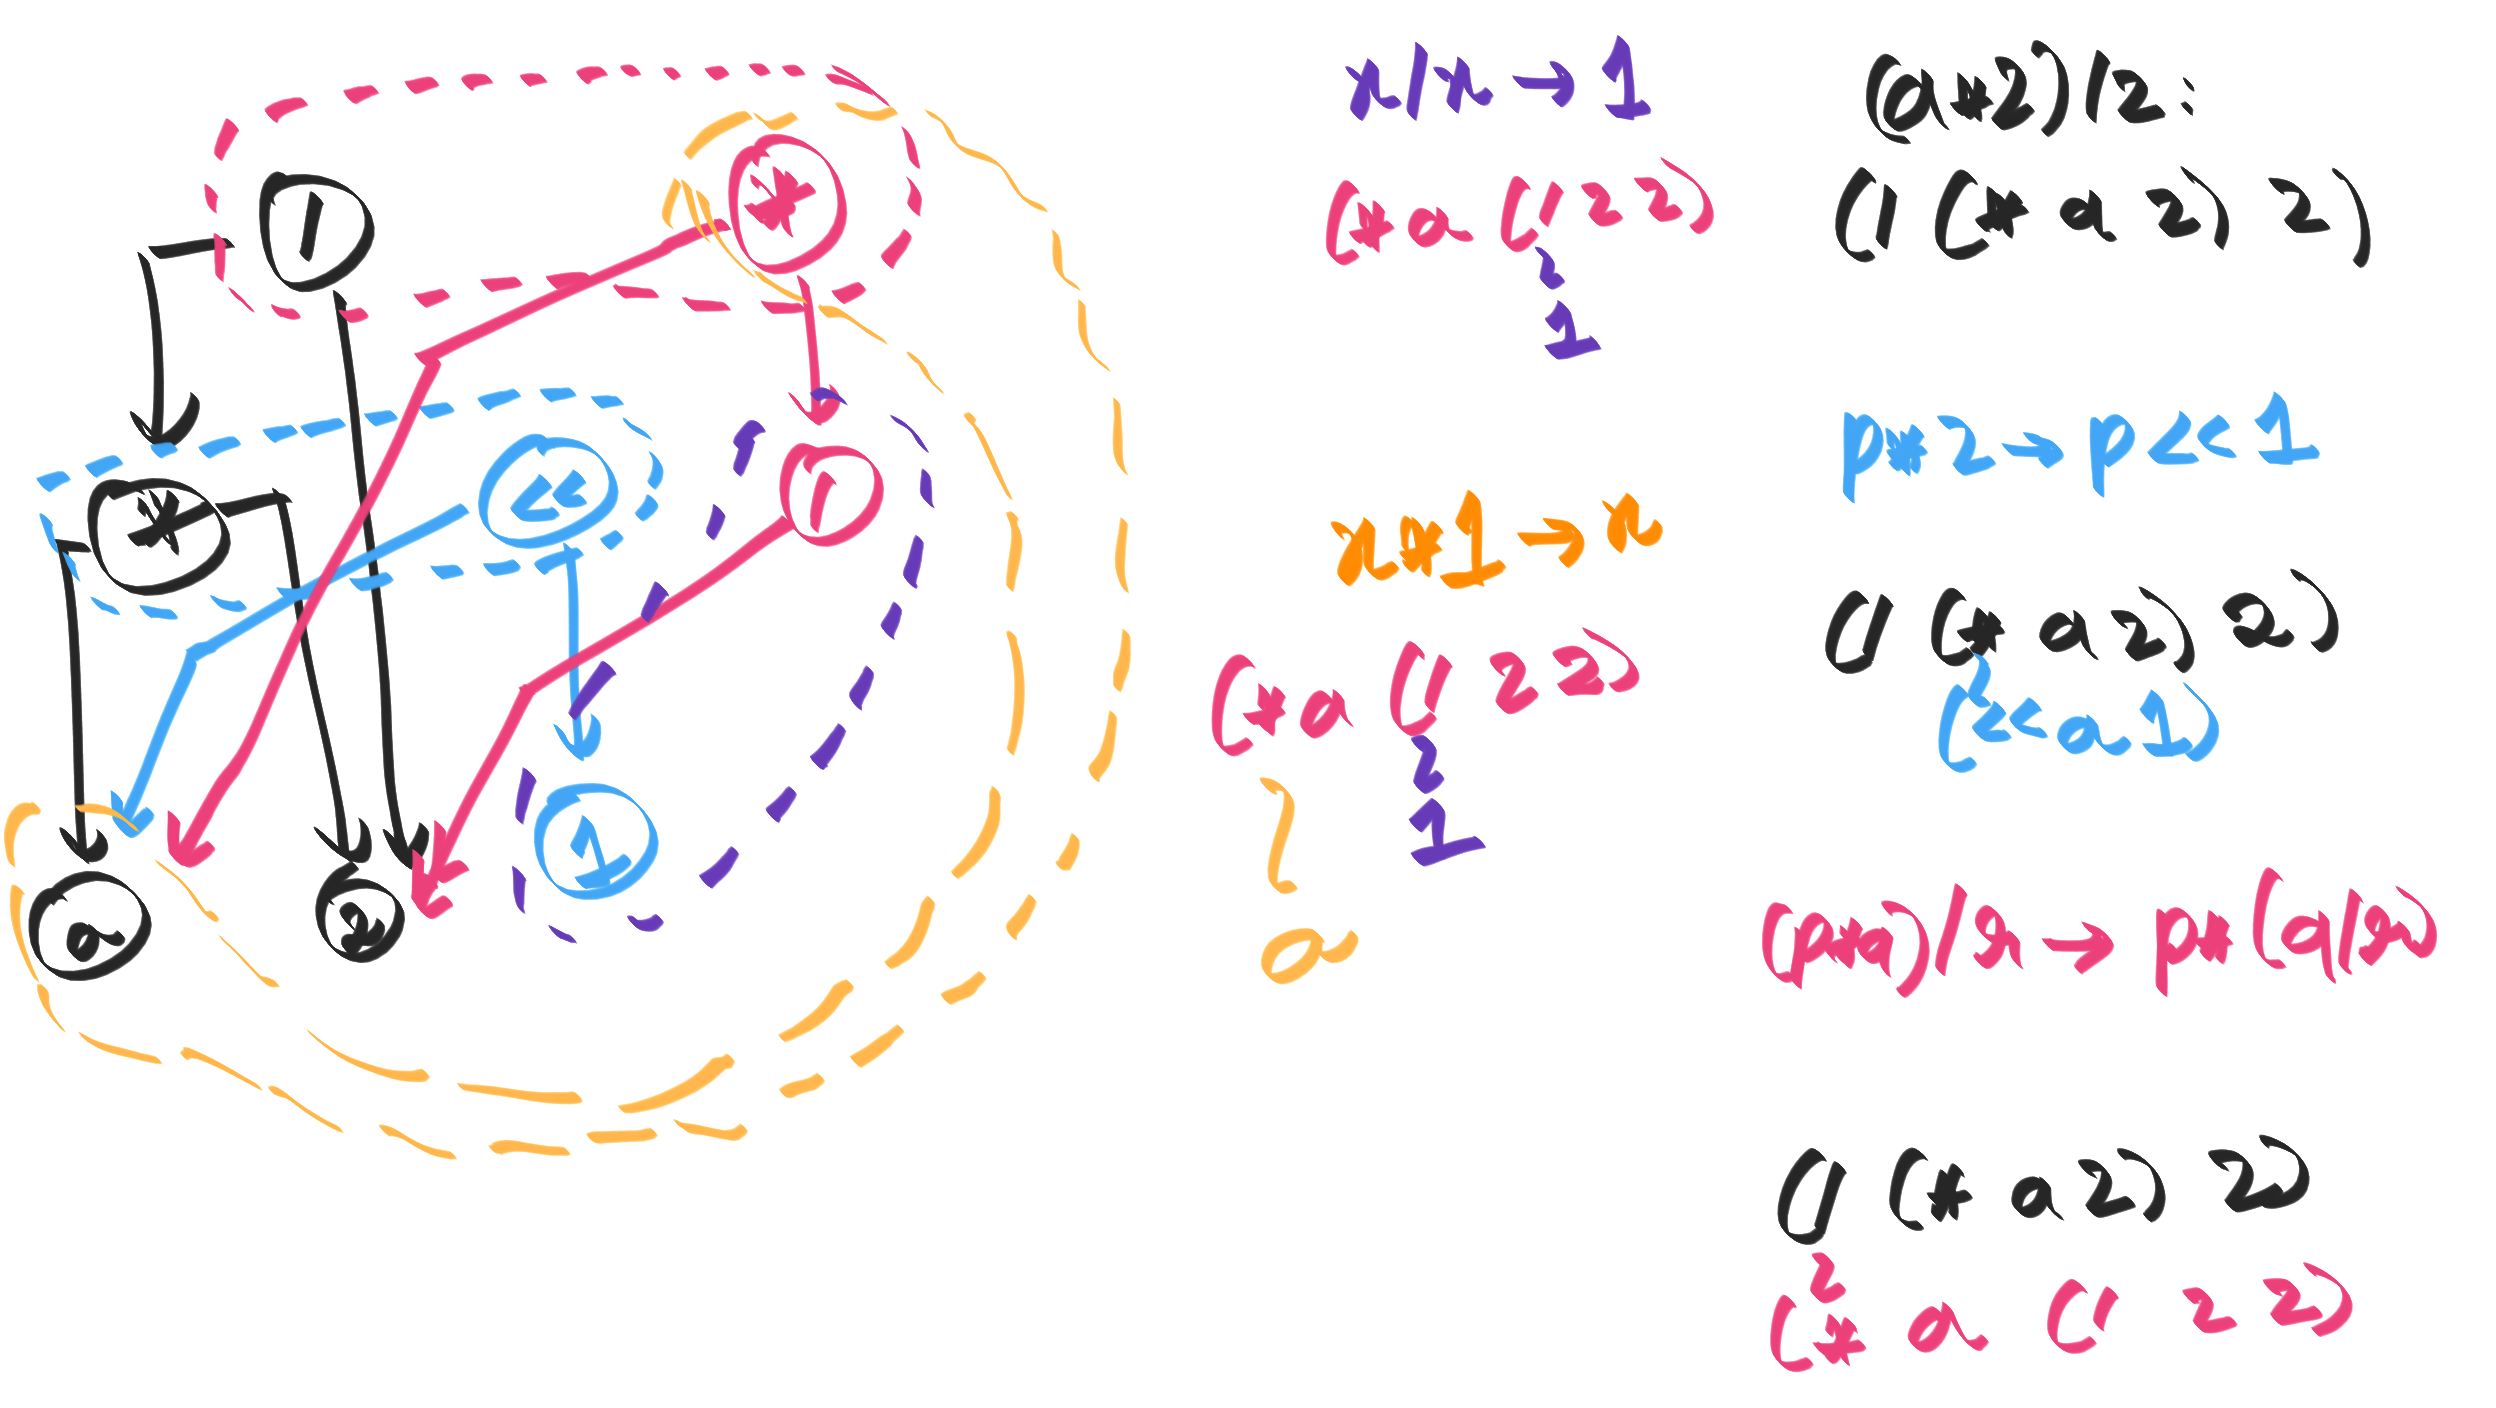
\includegraphics[width=\textwidth]{./eg-1-5.png}
\end{frame}


\begin{frame}[fragile]{\egg: Fast and extensible equality saturation (6)}
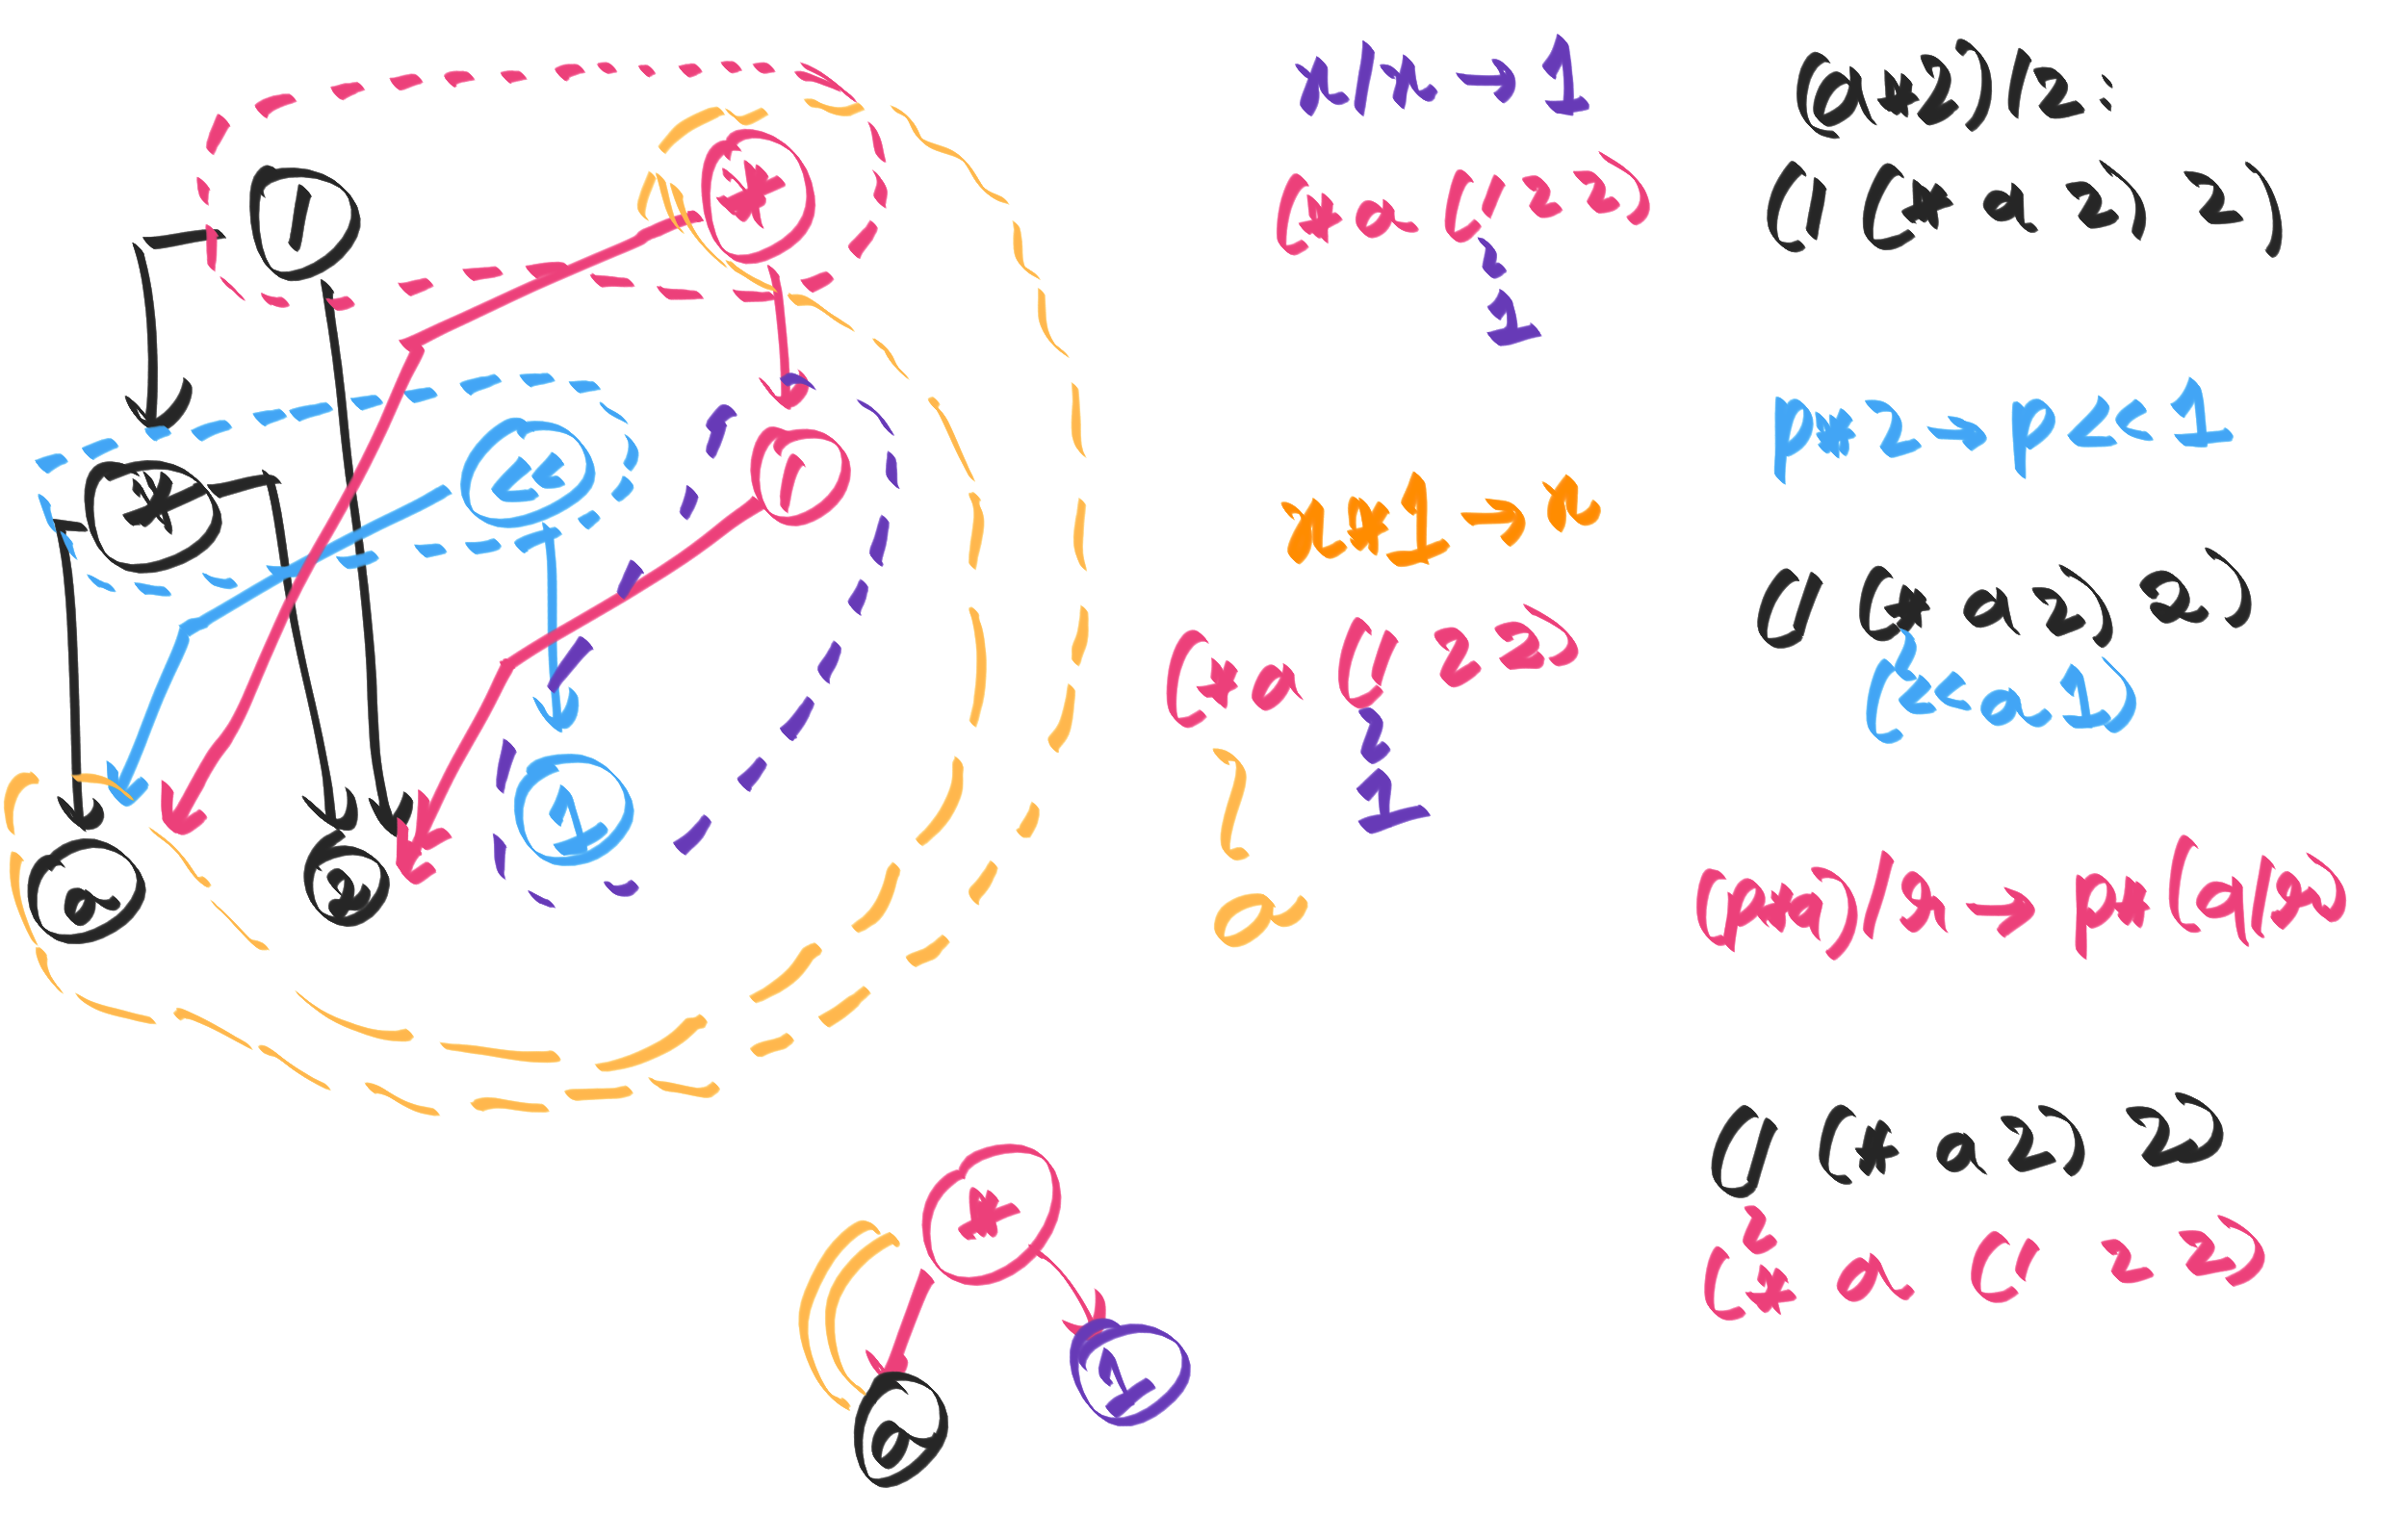
\includegraphics[width=\textwidth]{./eg-1-6.png}
\end{frame}

\begin{frame}[fragile]{\egg: Fast and extensible equality saturation (7)}
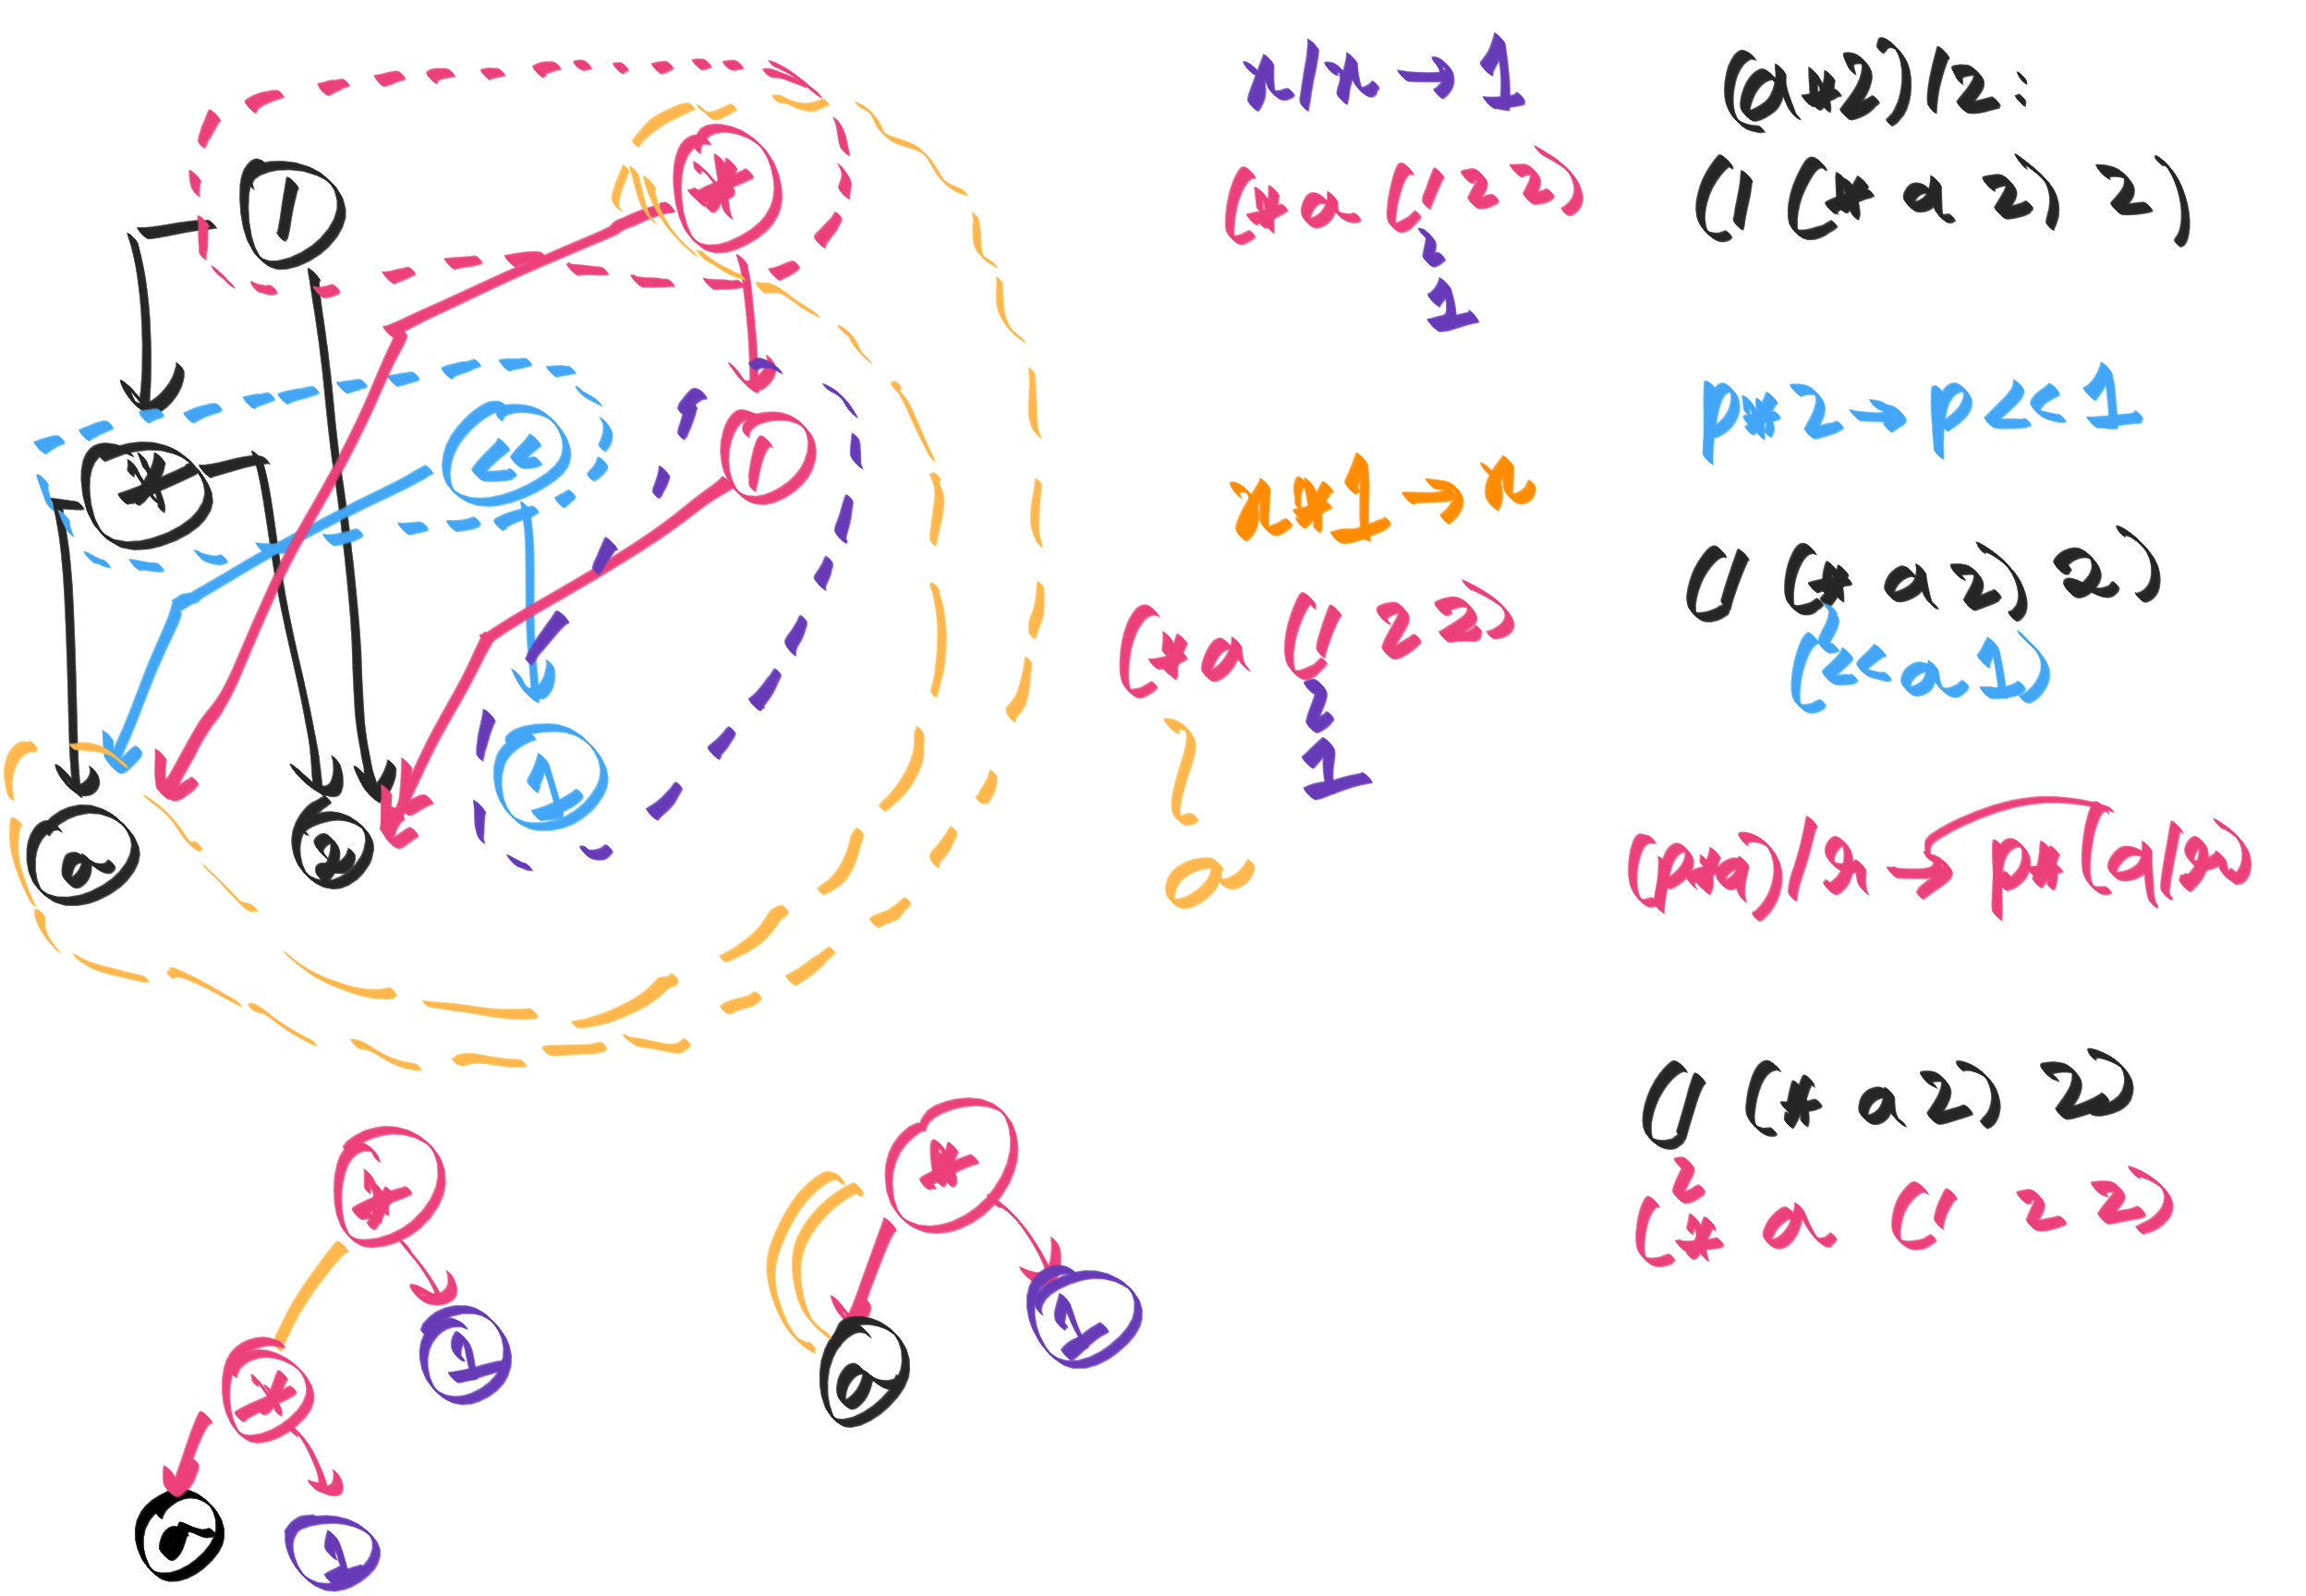
\includegraphics[width=\textwidth]{./eg-1-7.png}
\end{frame}


\begin{frame}[fragile]{\egg: Fast and extensible equality saturation (8)}
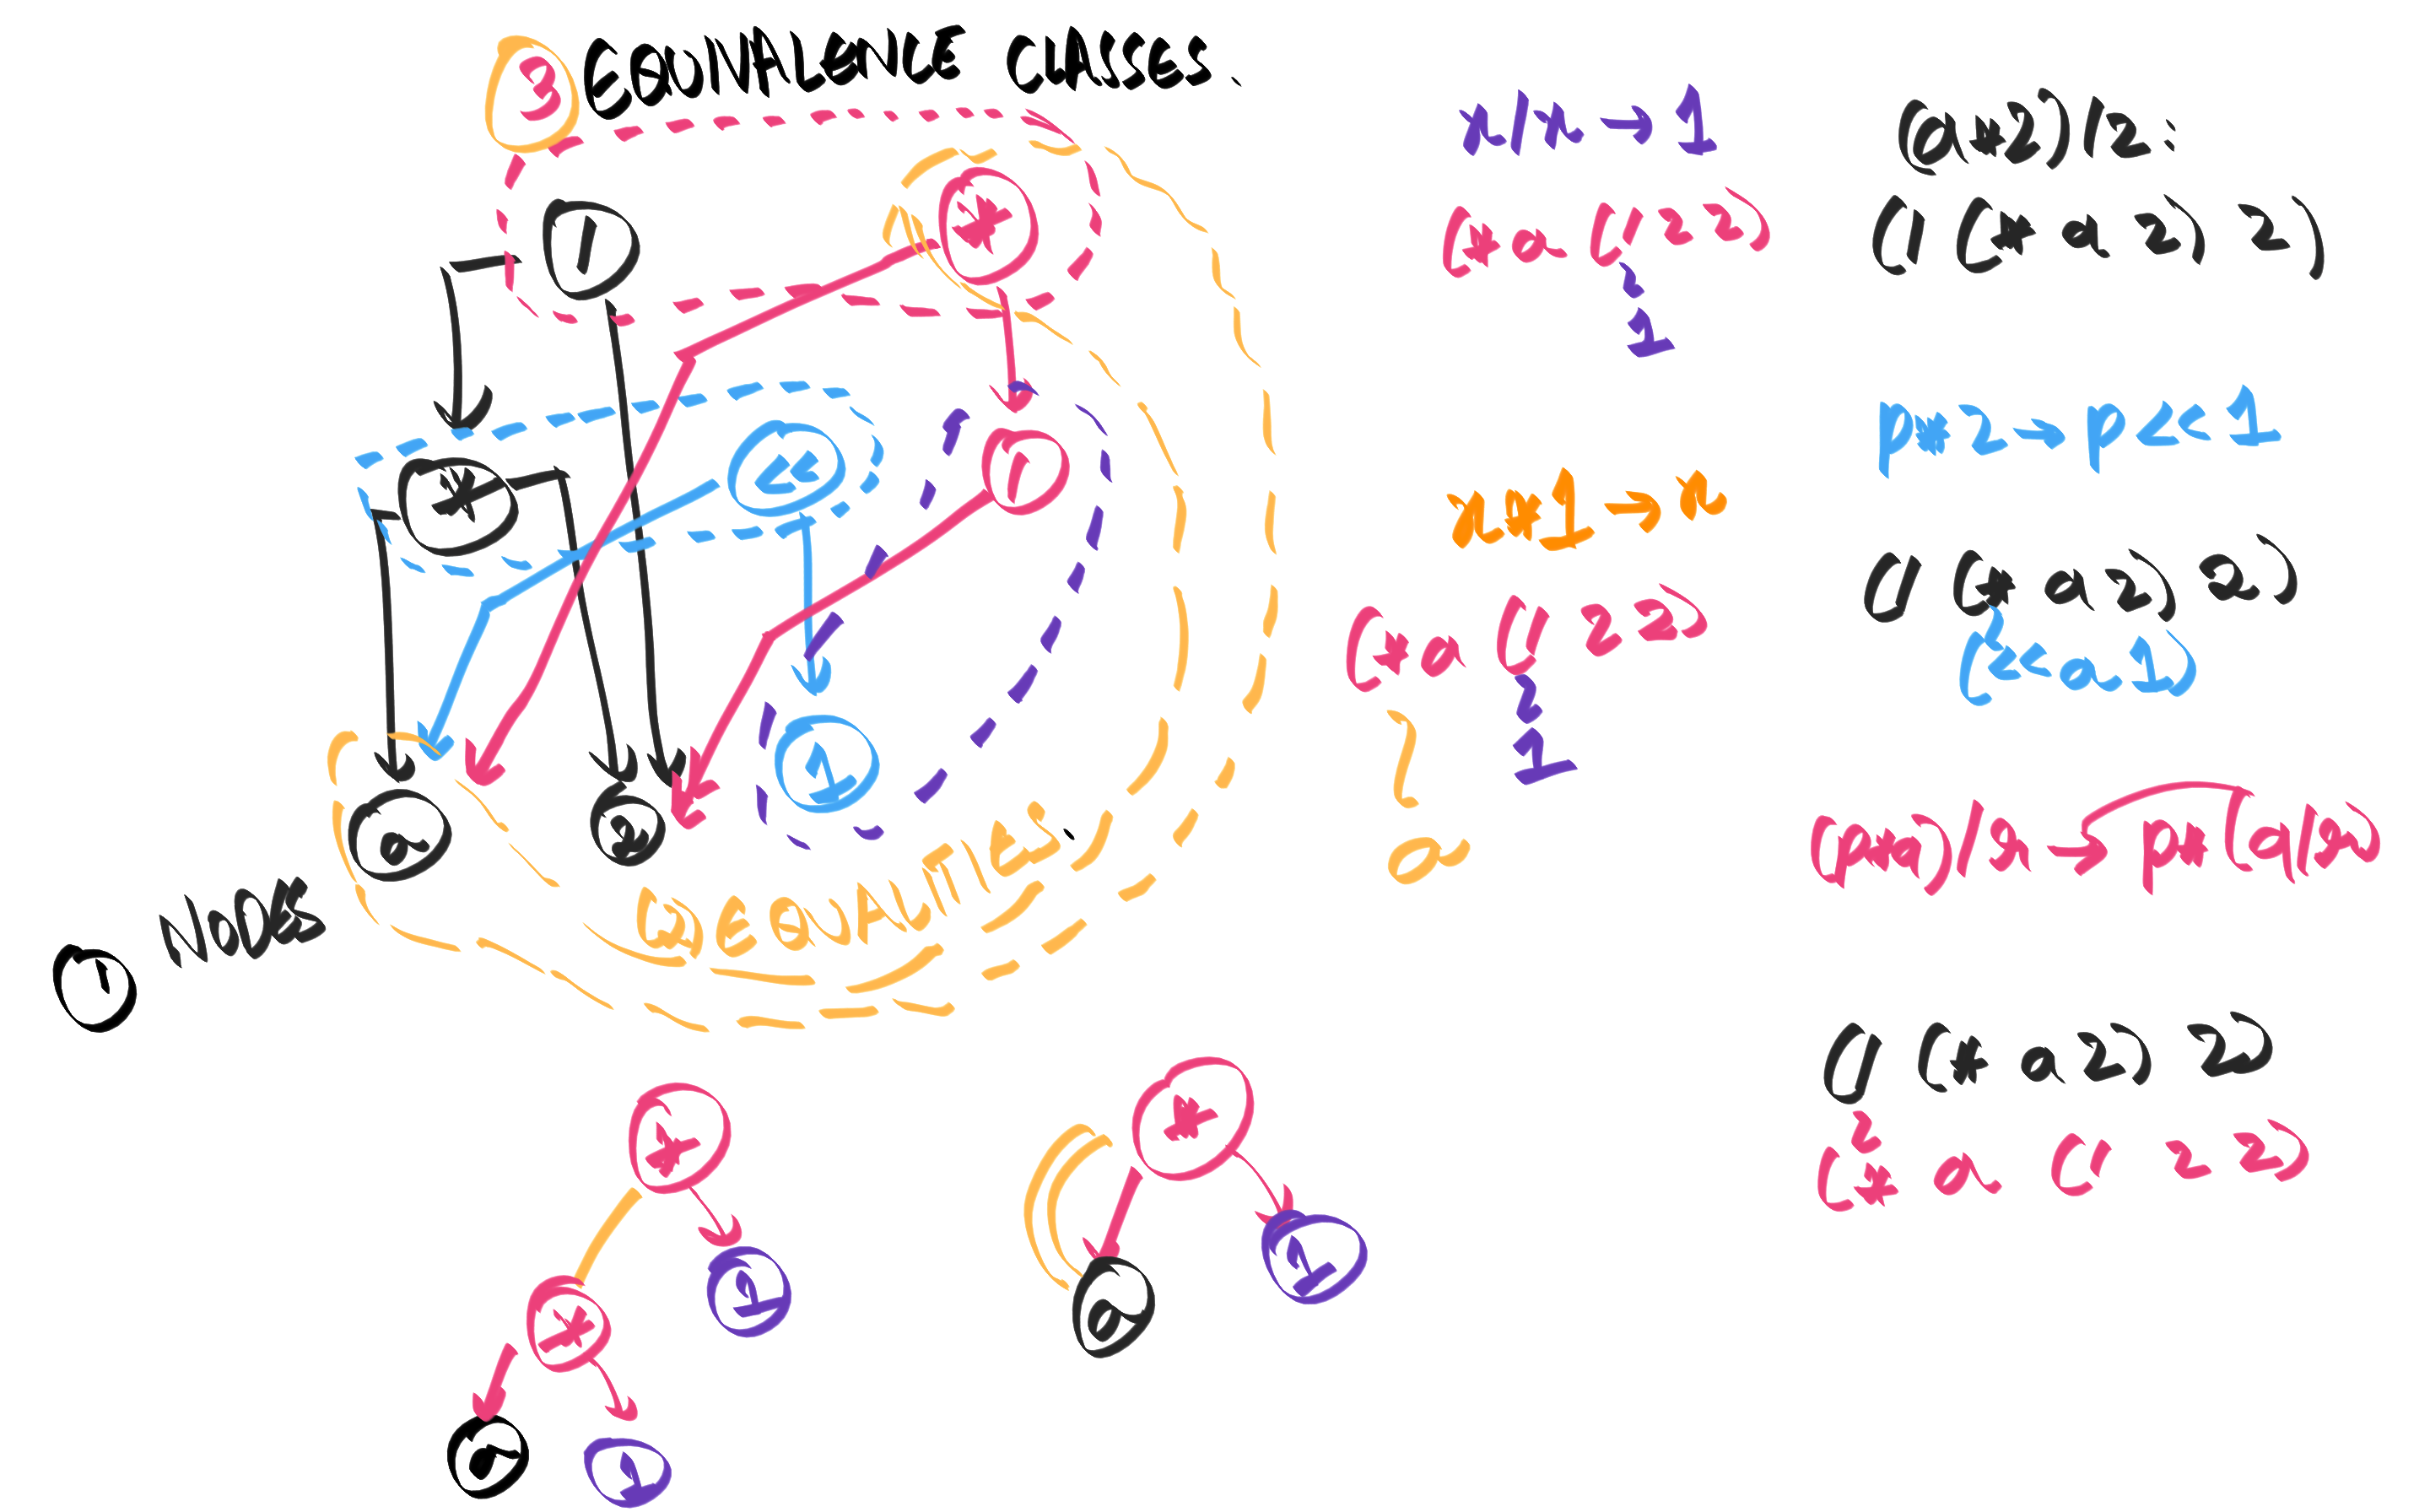
\includegraphics[width=\textwidth]{./eg-1-8.png}
\end{frame}


\begin{frame}{Evaluation: Herbie}
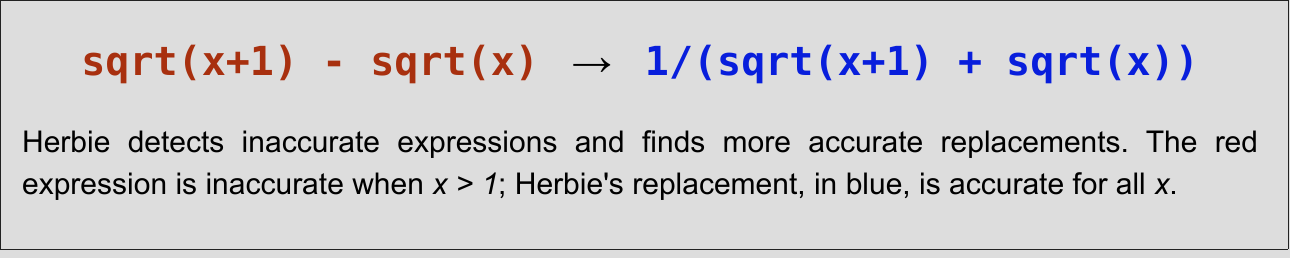
\includegraphics[width=\textwidth]{./herbie-sales-pitch.png}
\pause

$$
\sqrt{x+1}-\sqrt{x} =
\frac{(\sqrt{x+1}-\sqrt{x})(\sqrt{x+1}+\sqrt{x})}{\sqrt{x+1}+\sqrt{x}}
= \frac{(x+1)-x}{\sqrt{x+1}+\sqrt{x}} = \frac{1}{(\sqrt{x+1}+\sqrt{x})}
$$
\pause
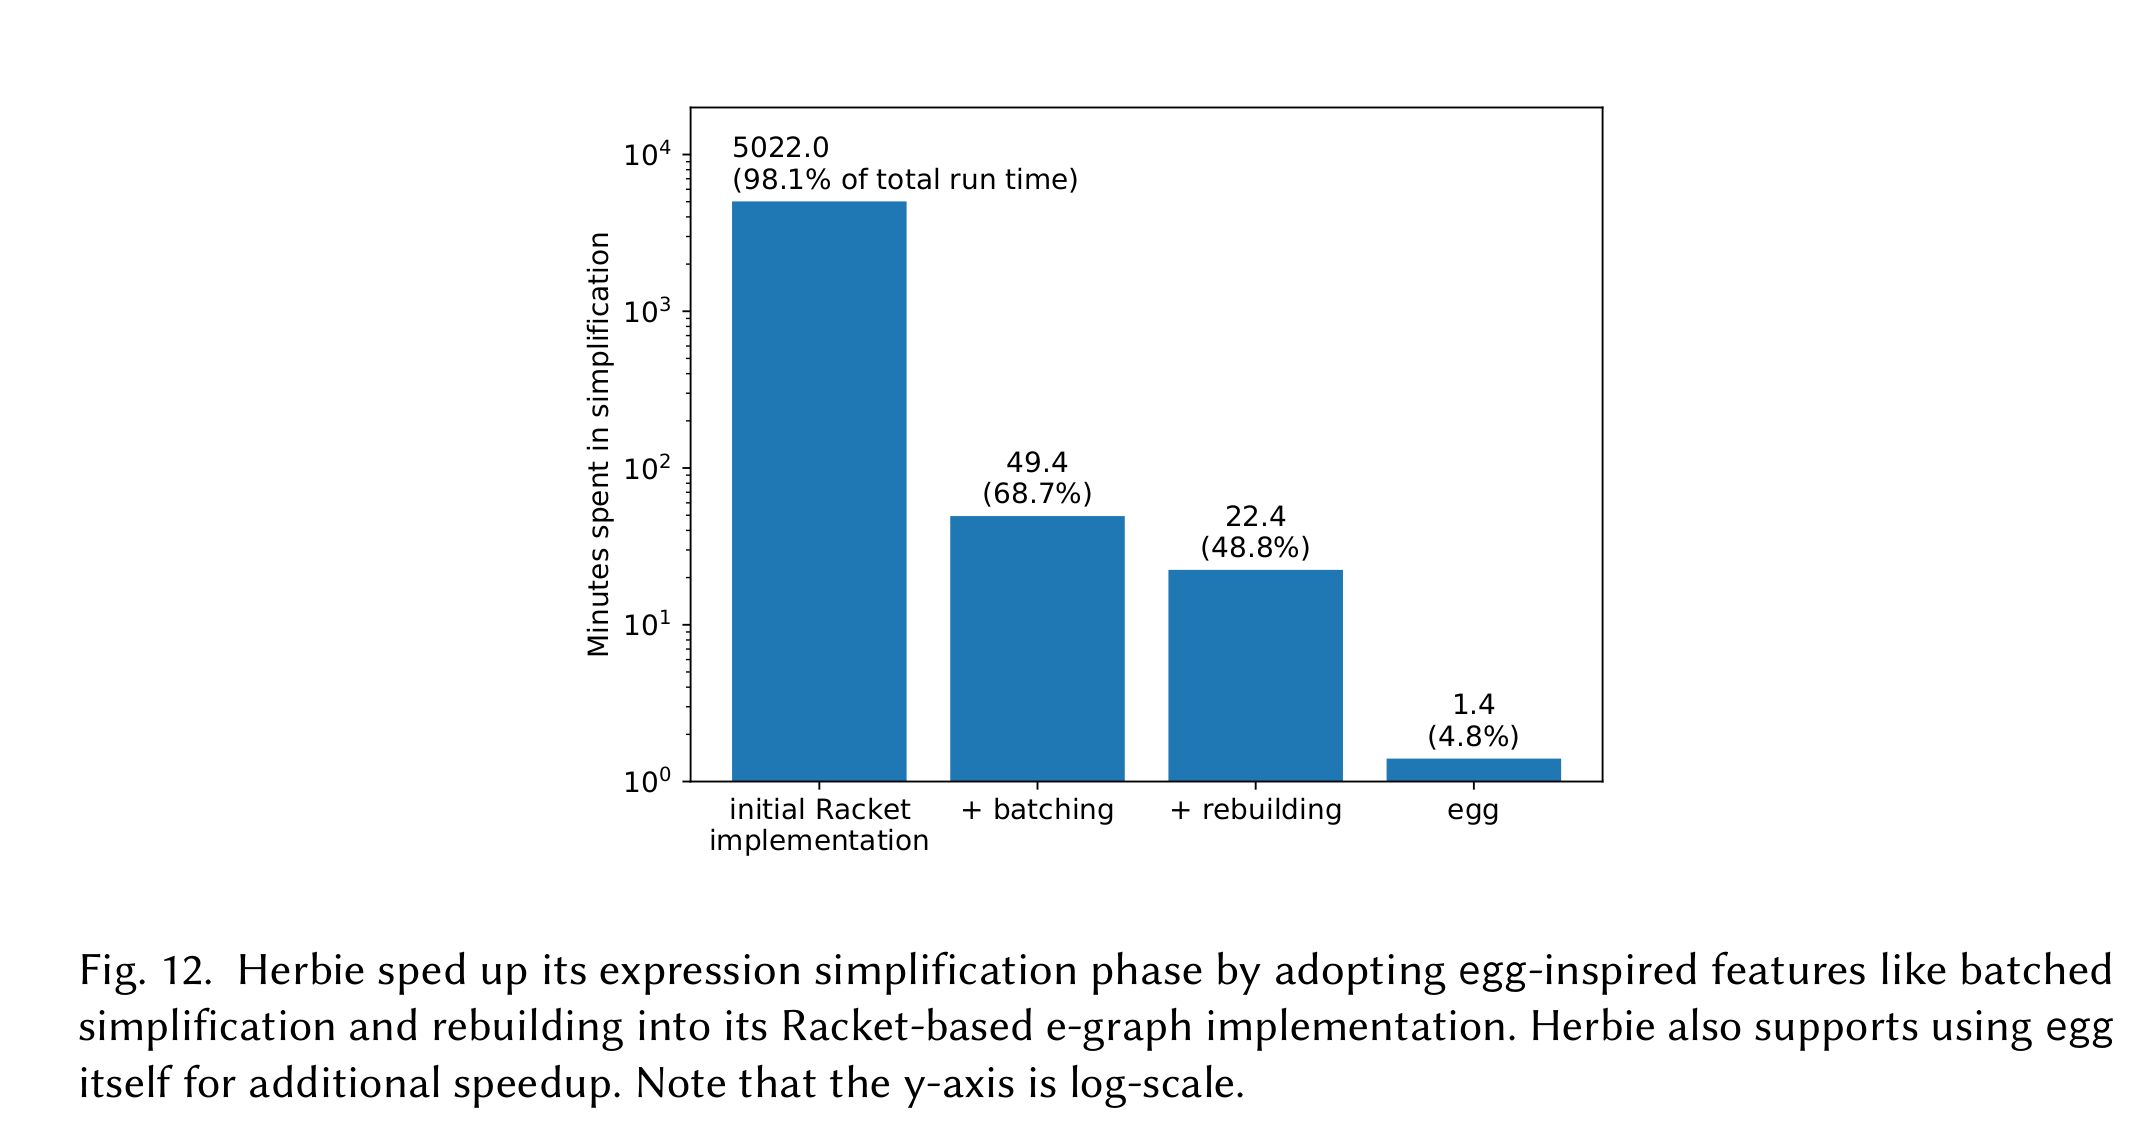
\includegraphics[width=0.8\textwidth]{./herbie-speedup.png}

\end{frame}

\begin{frame}[fragile]{Herbie: Using \egg --- Analysis and rewrite}
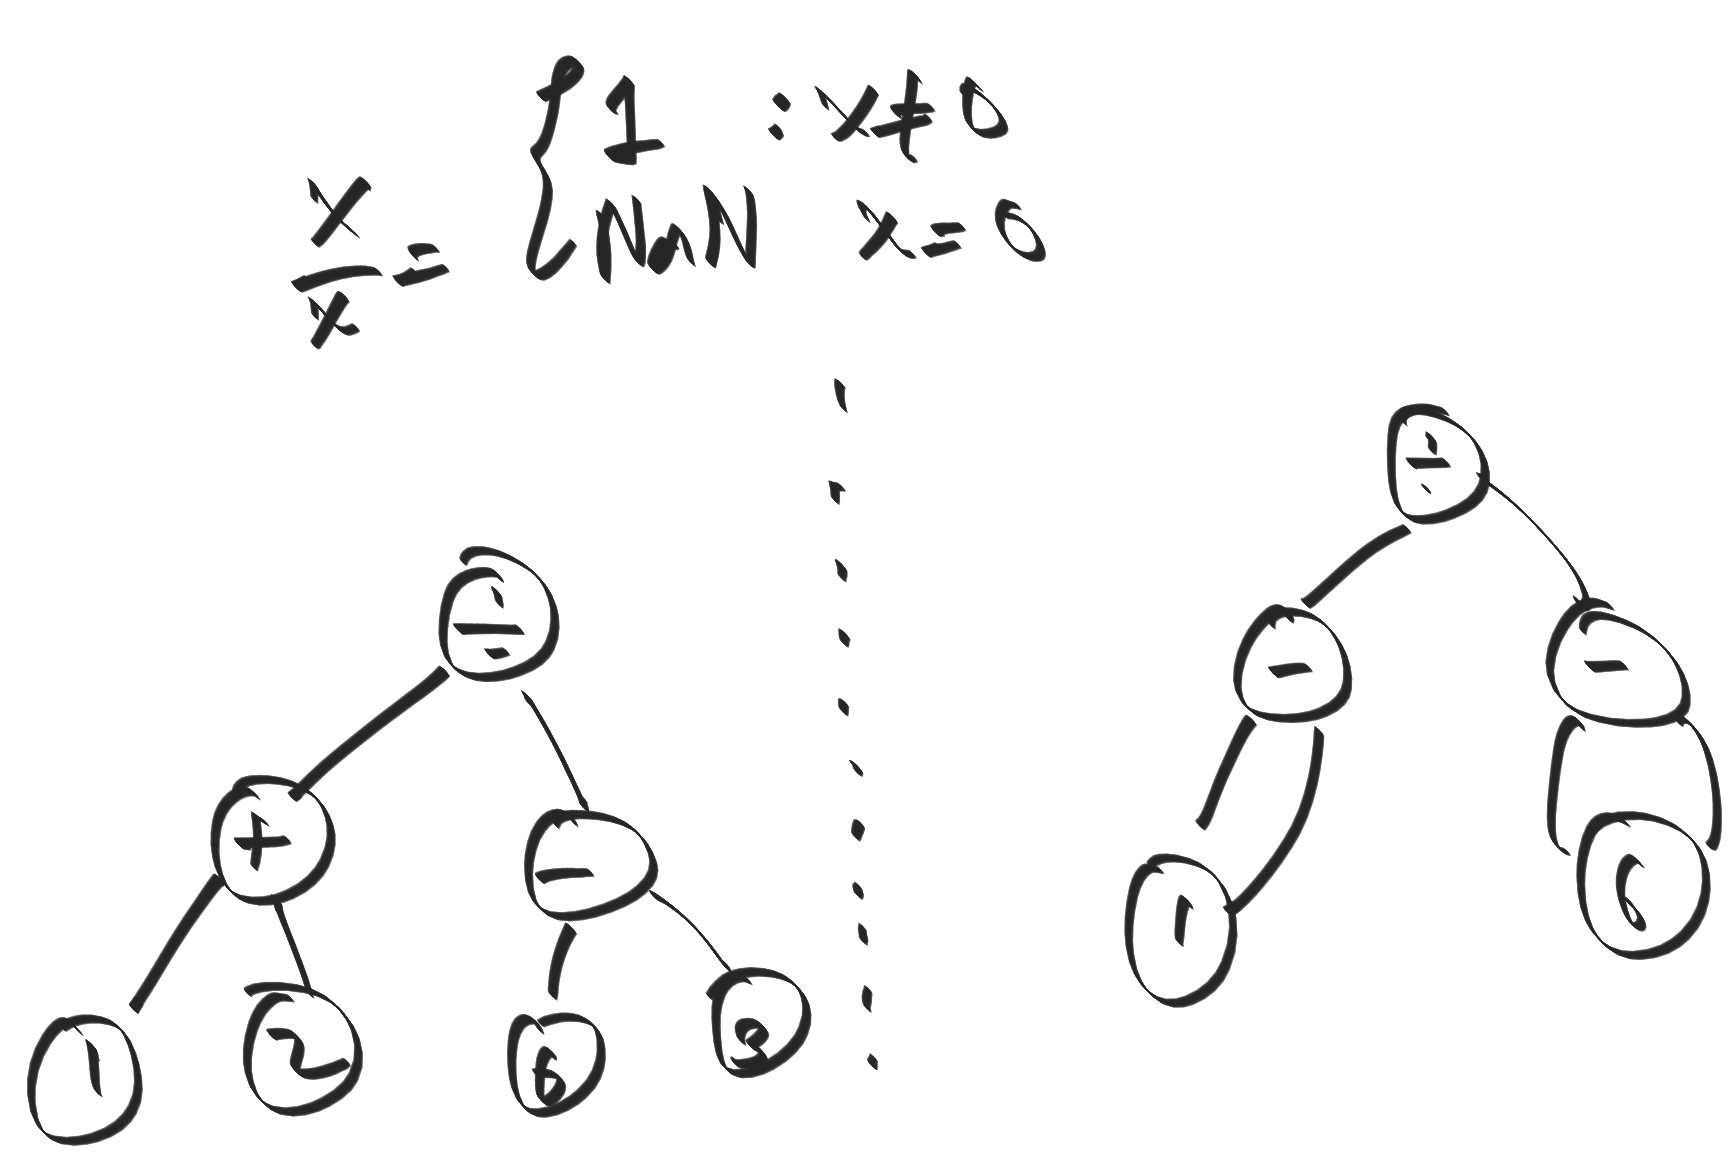
\includegraphics[width=\textwidth]{./rewrite-1.png}
\end{frame}


\begin{frame}[fragile]{Herbie: Using \egg --- Analysis and rewrite}
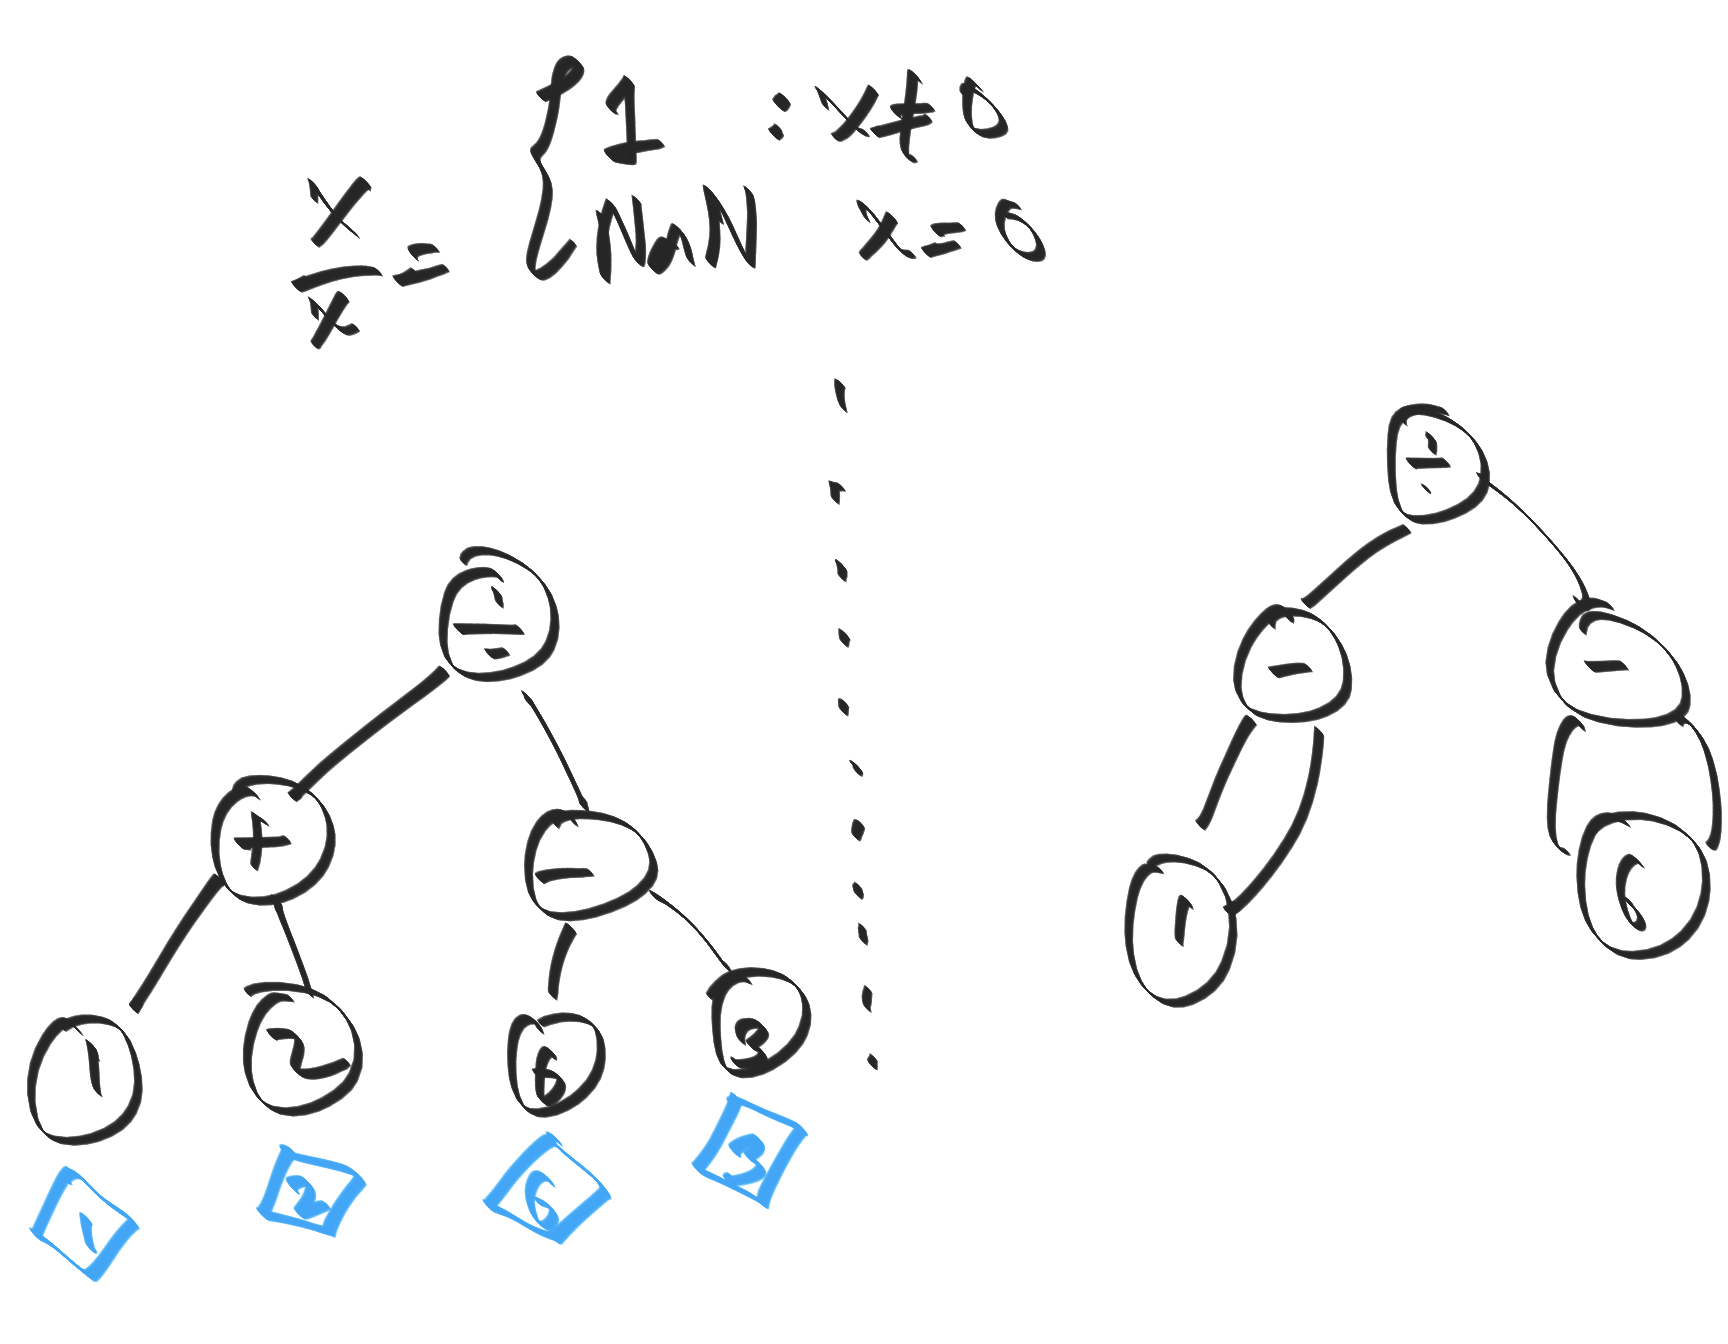
\includegraphics[width=\textwidth]{./rewrite-2.png}
\end{frame}


\begin{frame}[fragile]{Herbie: Using \egg --- Analysis and rewrite}
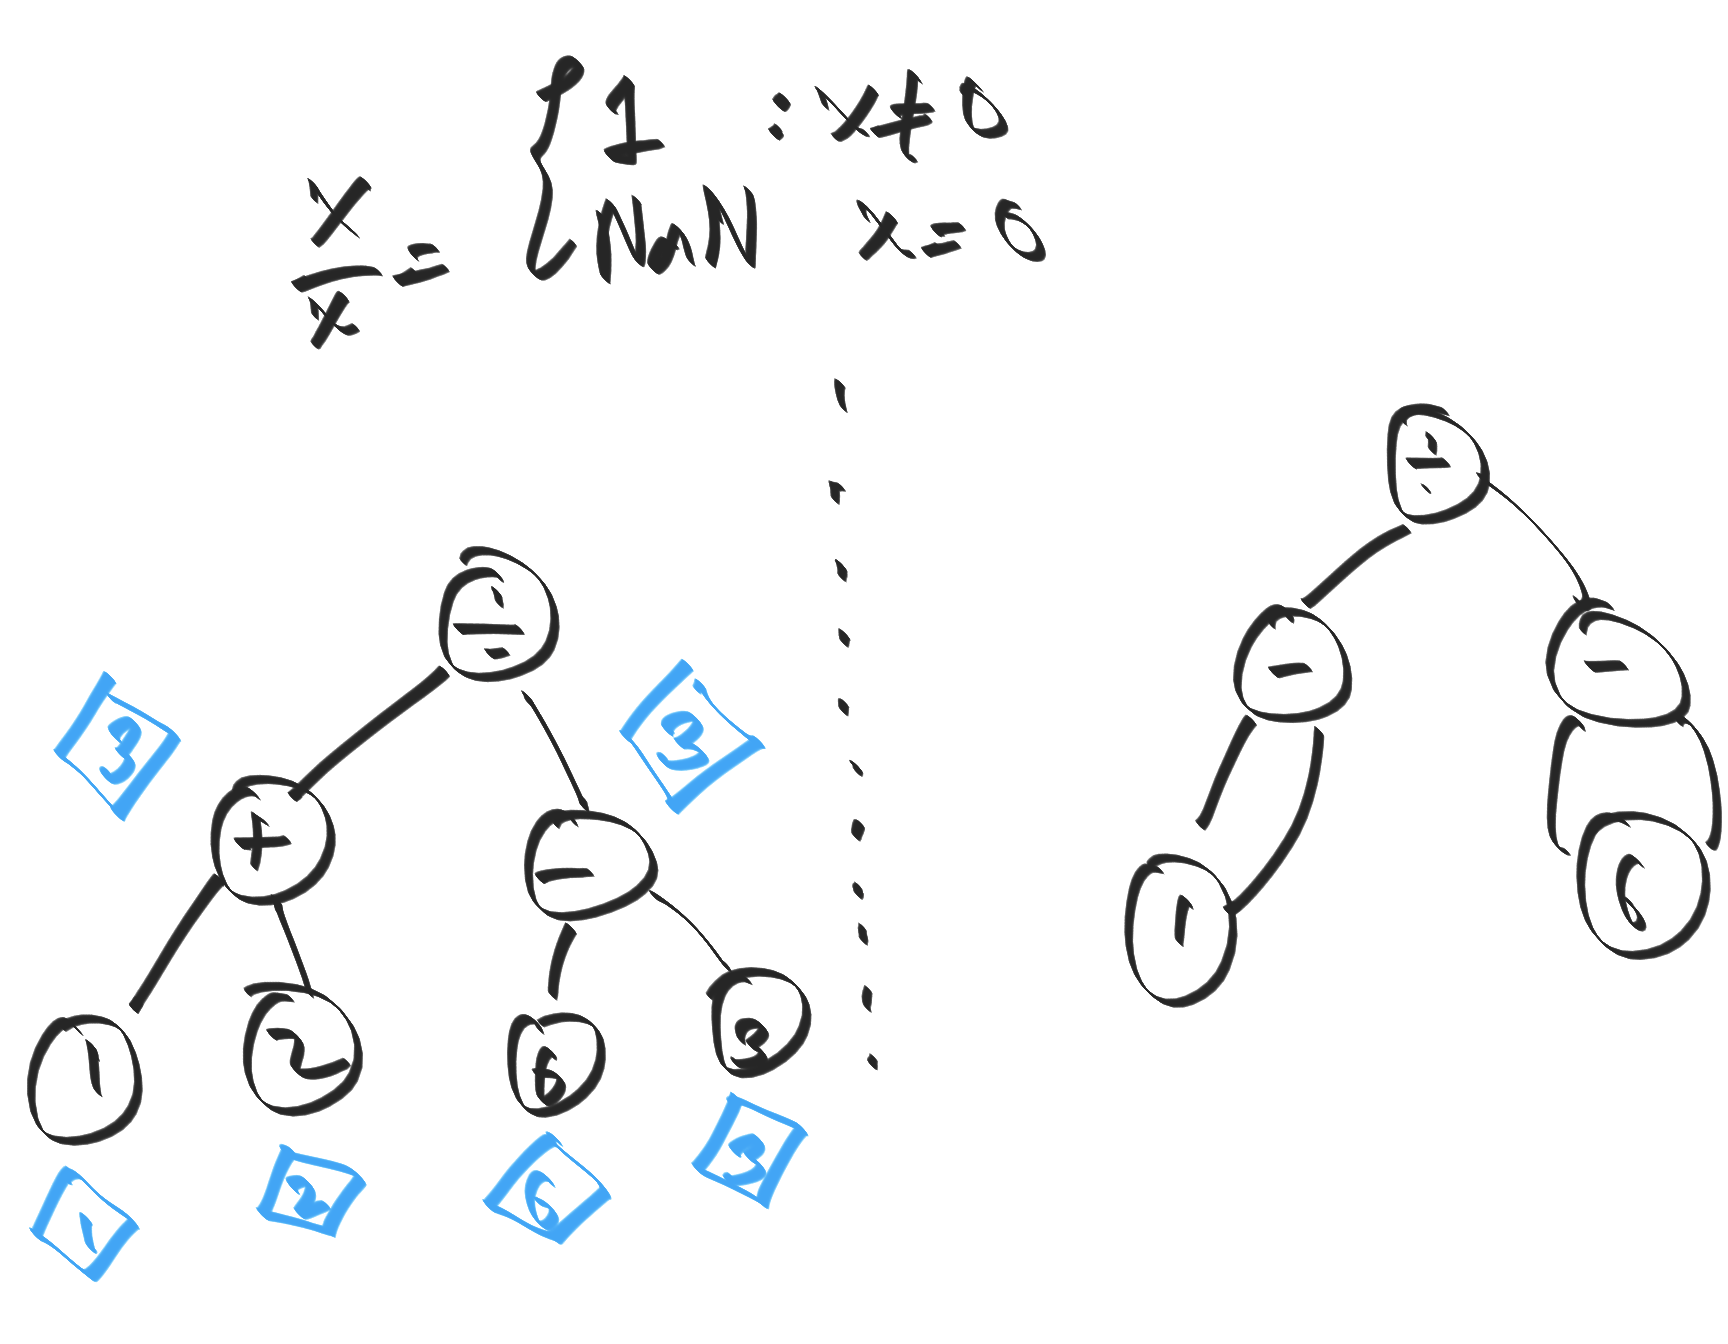
\includegraphics[width=\textwidth]{./rewrite-3.png}
\end{frame}


\begin{frame}[fragile]{Herbie: Using \egg --- Analysis and rewrite}
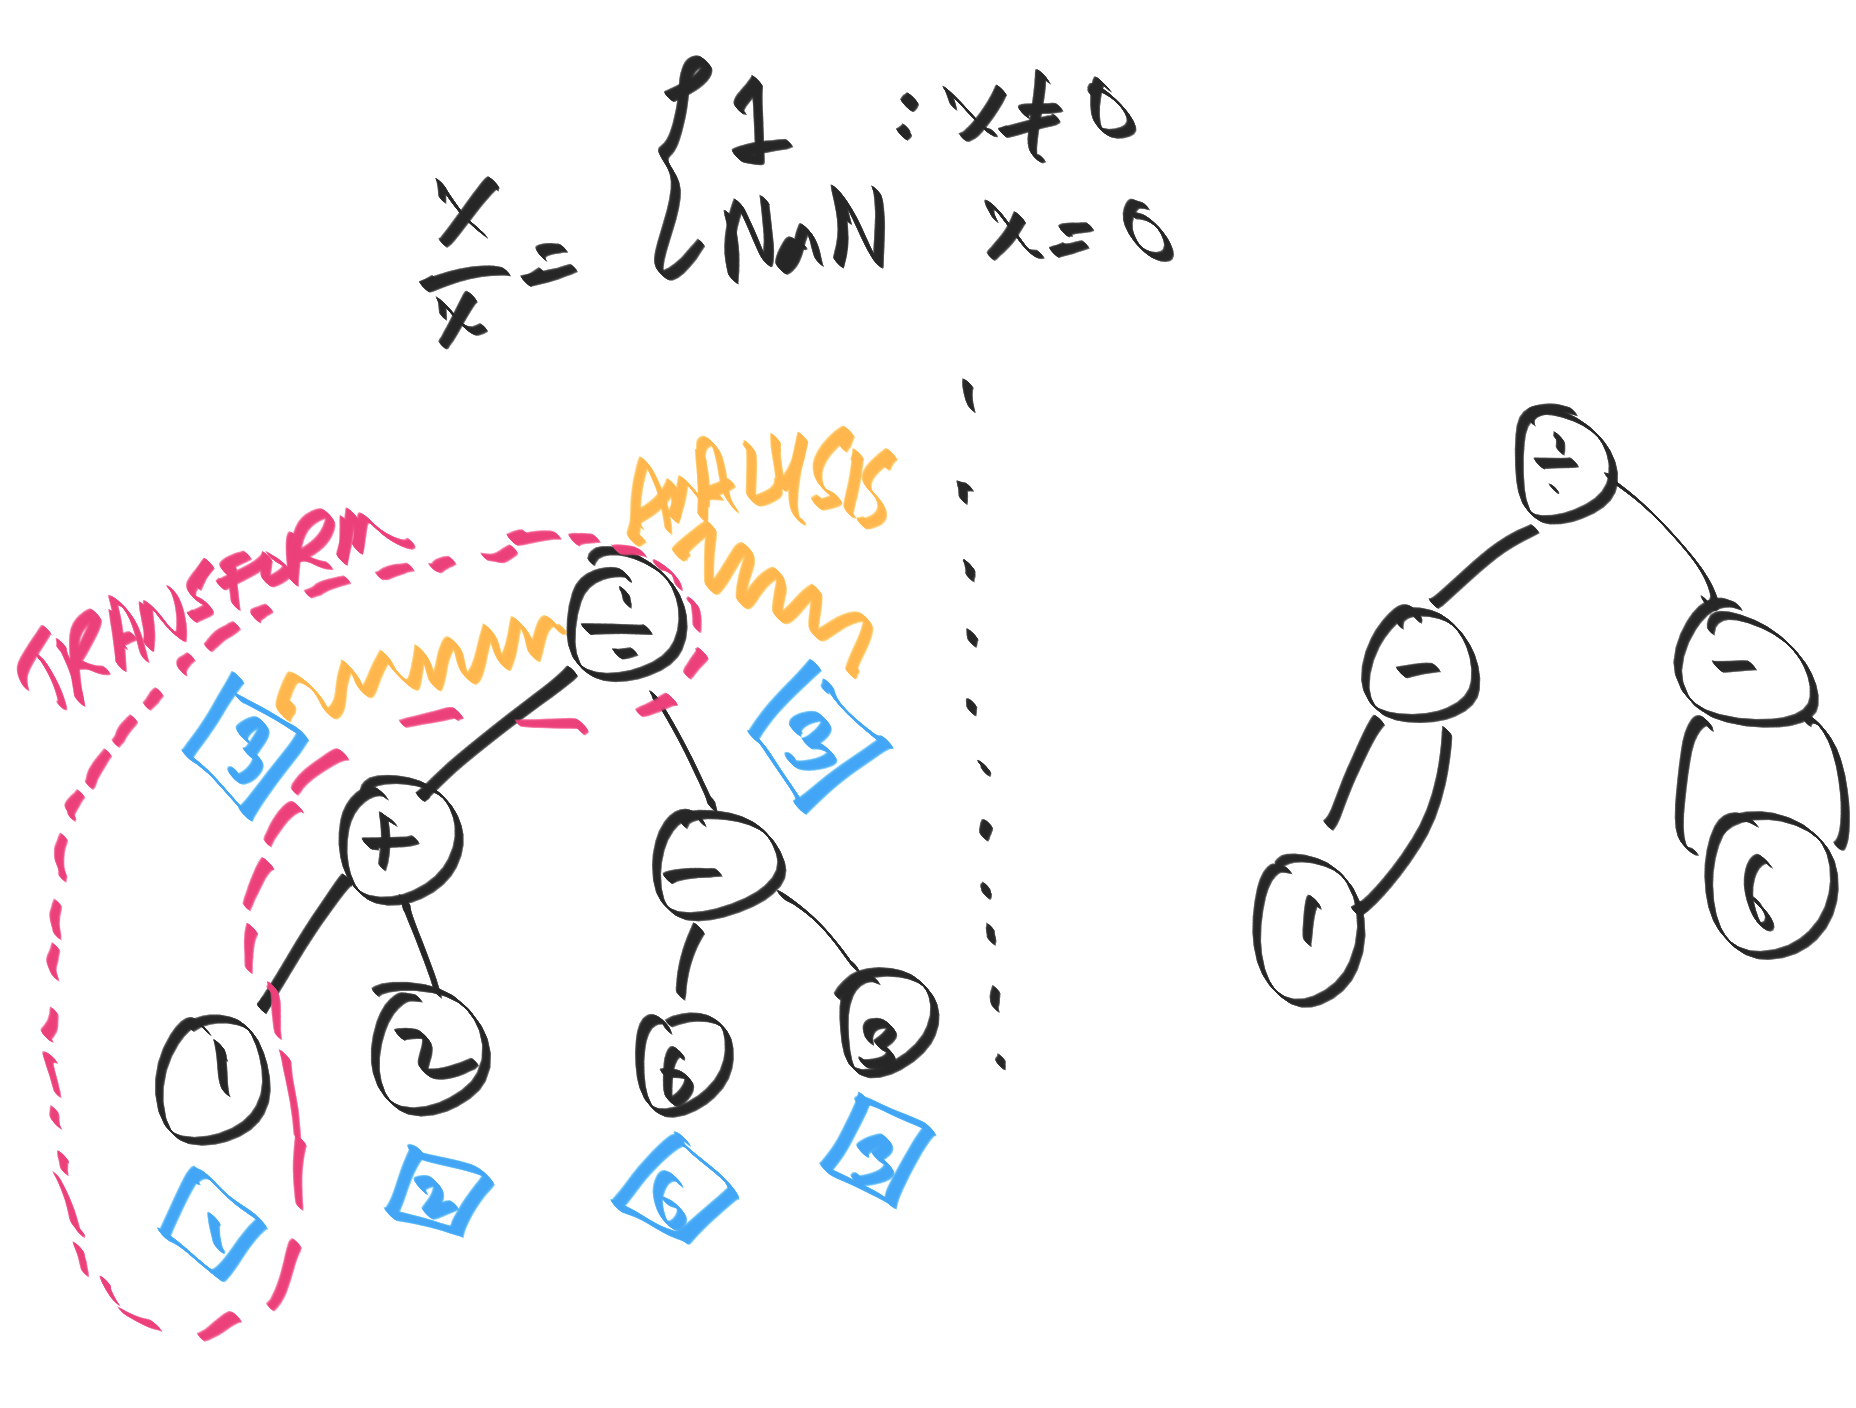
\includegraphics[width=\textwidth]{./rewrite-4.png}
\end{frame}


\begin{frame}[fragile]{Herbie: Using \egg --- Analysis and rewrite}
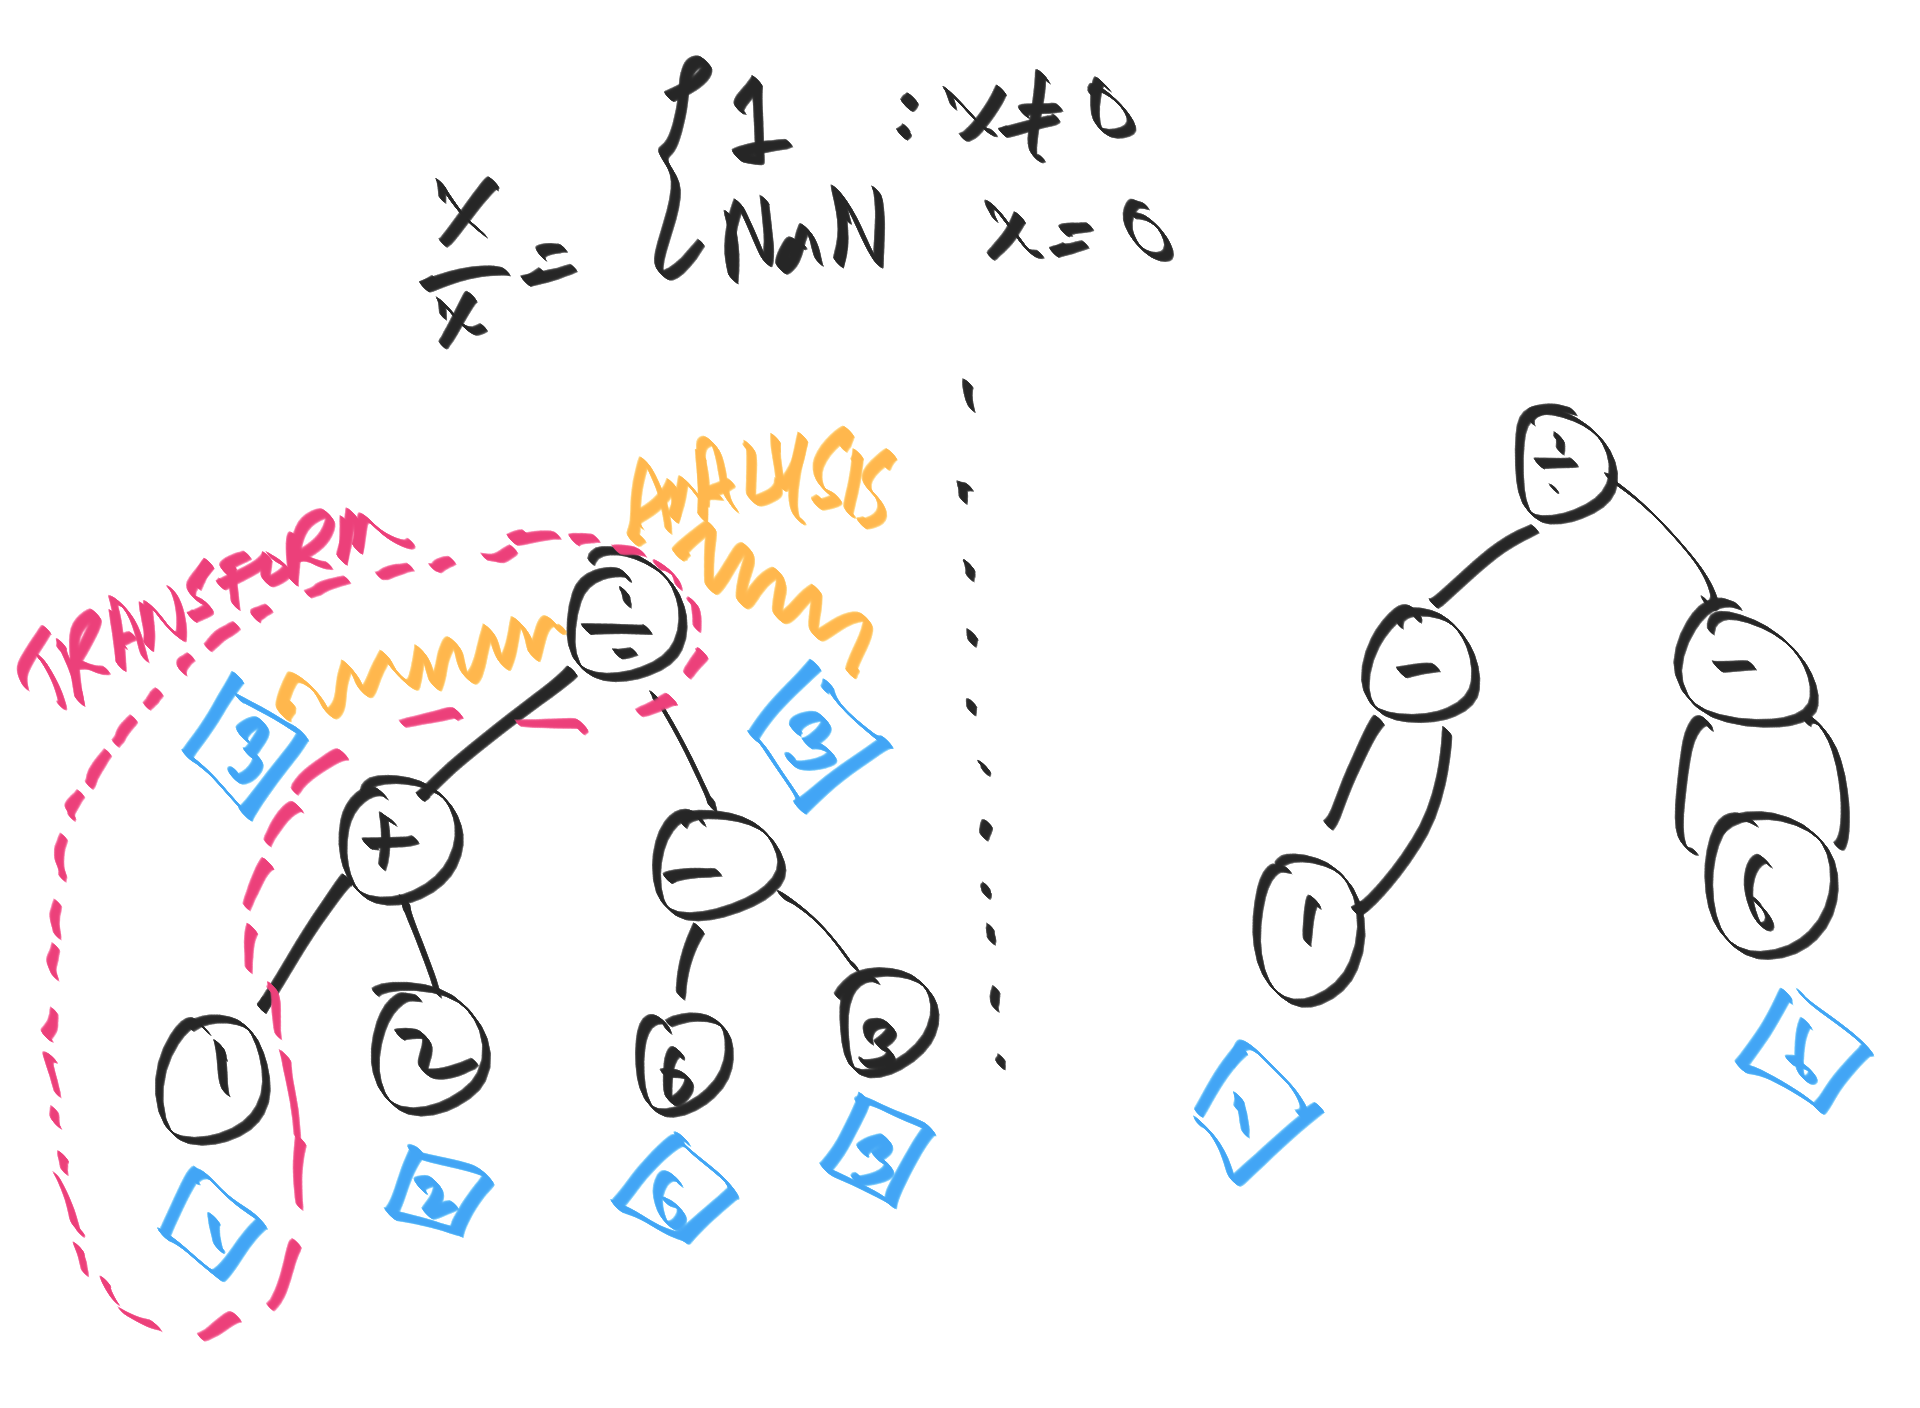
\includegraphics[width=\textwidth]{./rewrite-5.png}
\end{frame}


\begin{frame}[fragile]{Herbie: Using \egg --- Analysis and rewrite}
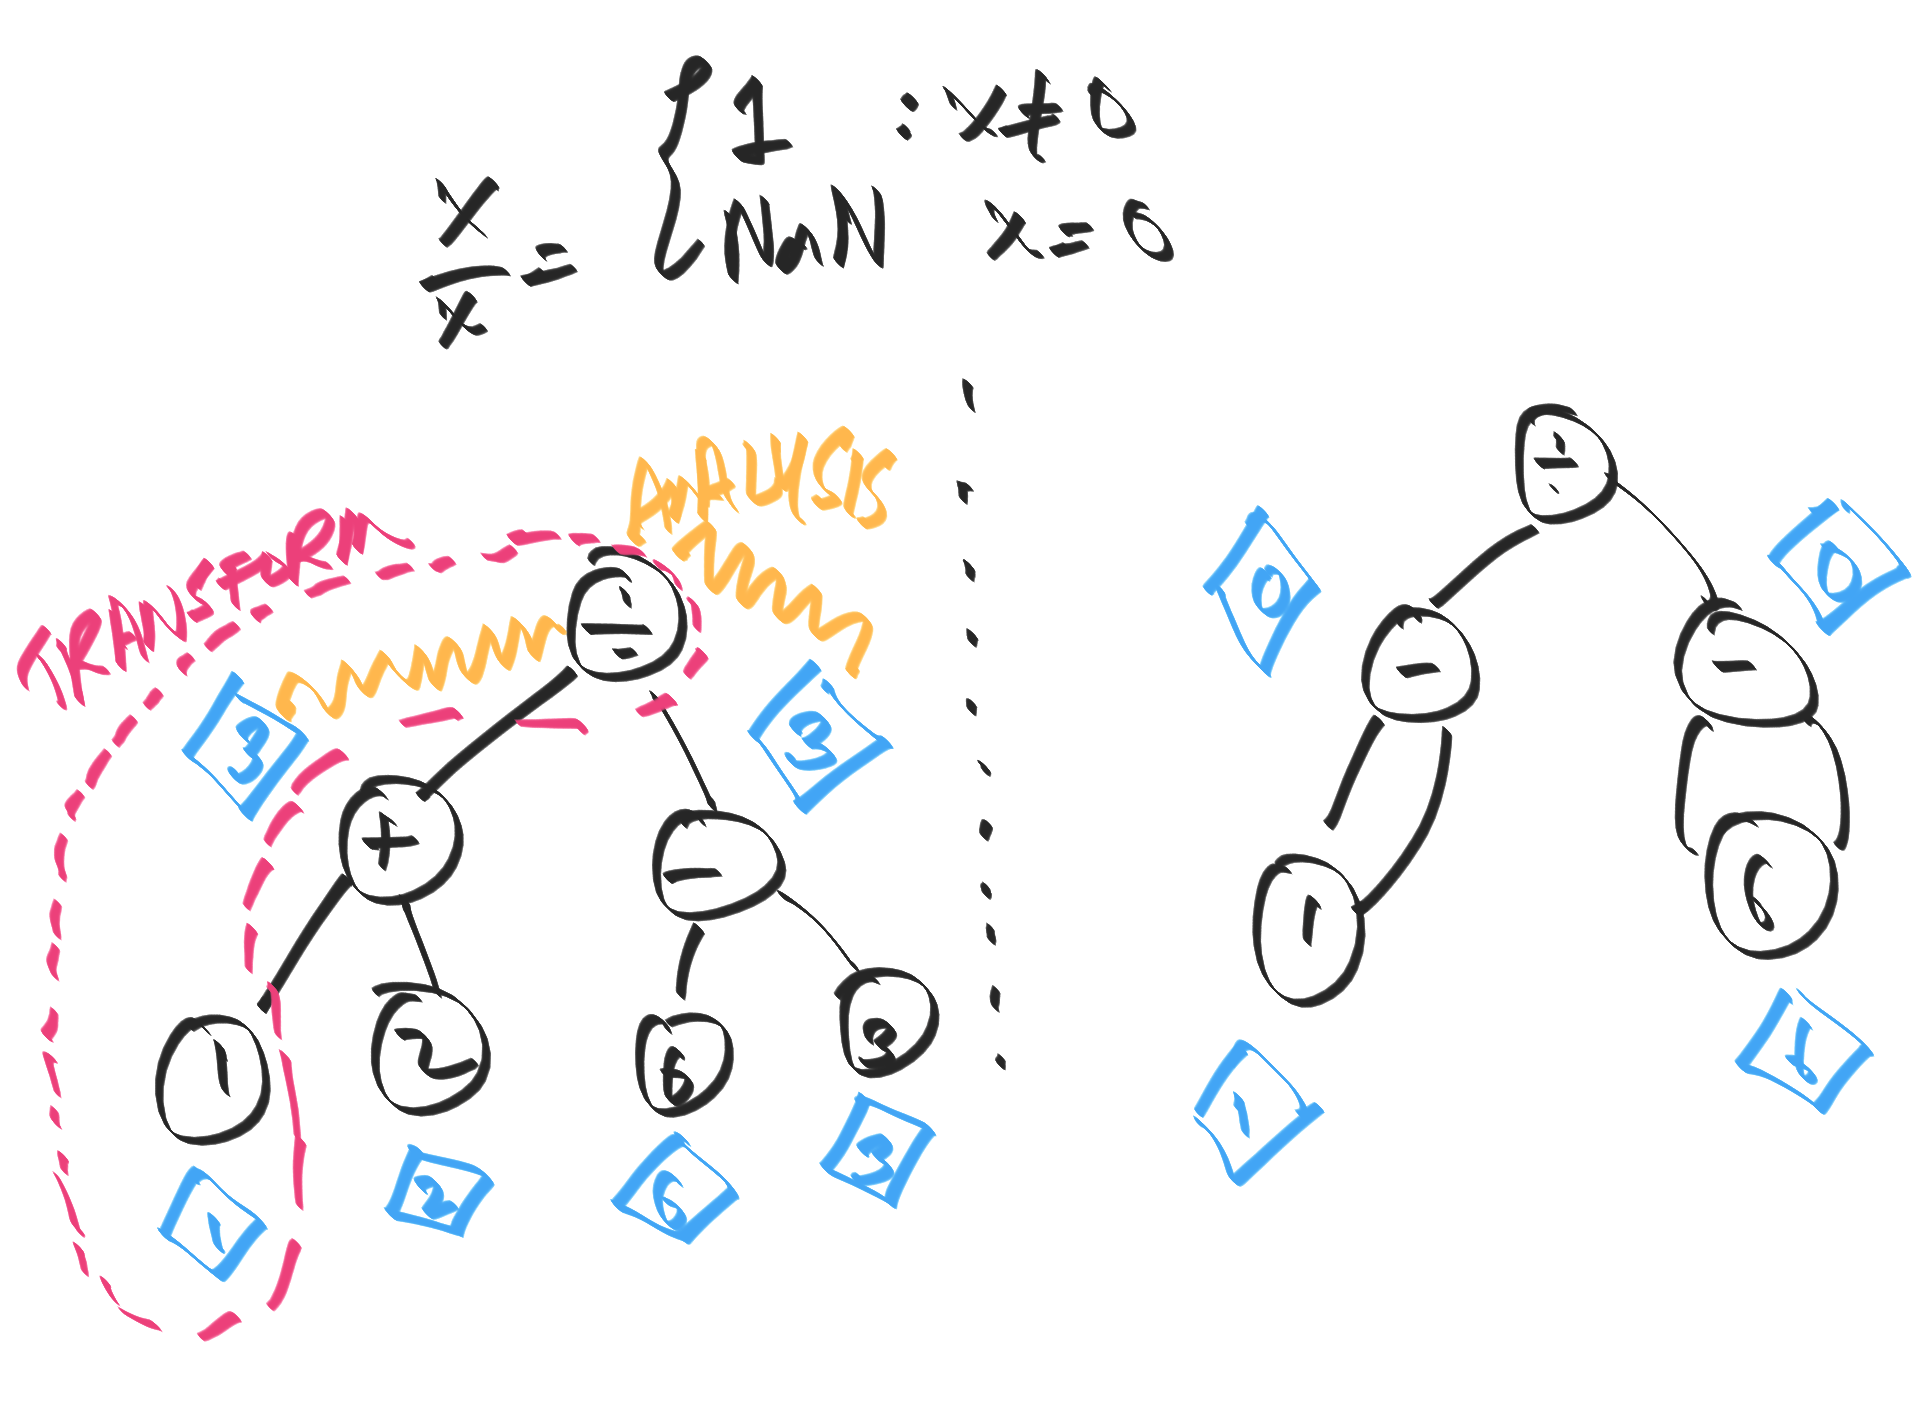
\includegraphics[width=\textwidth]{./rewrite-6.png}
\end{frame}


\begin{frame}[fragile]{Herbie: Using \egg --- Analysis and rewrite}
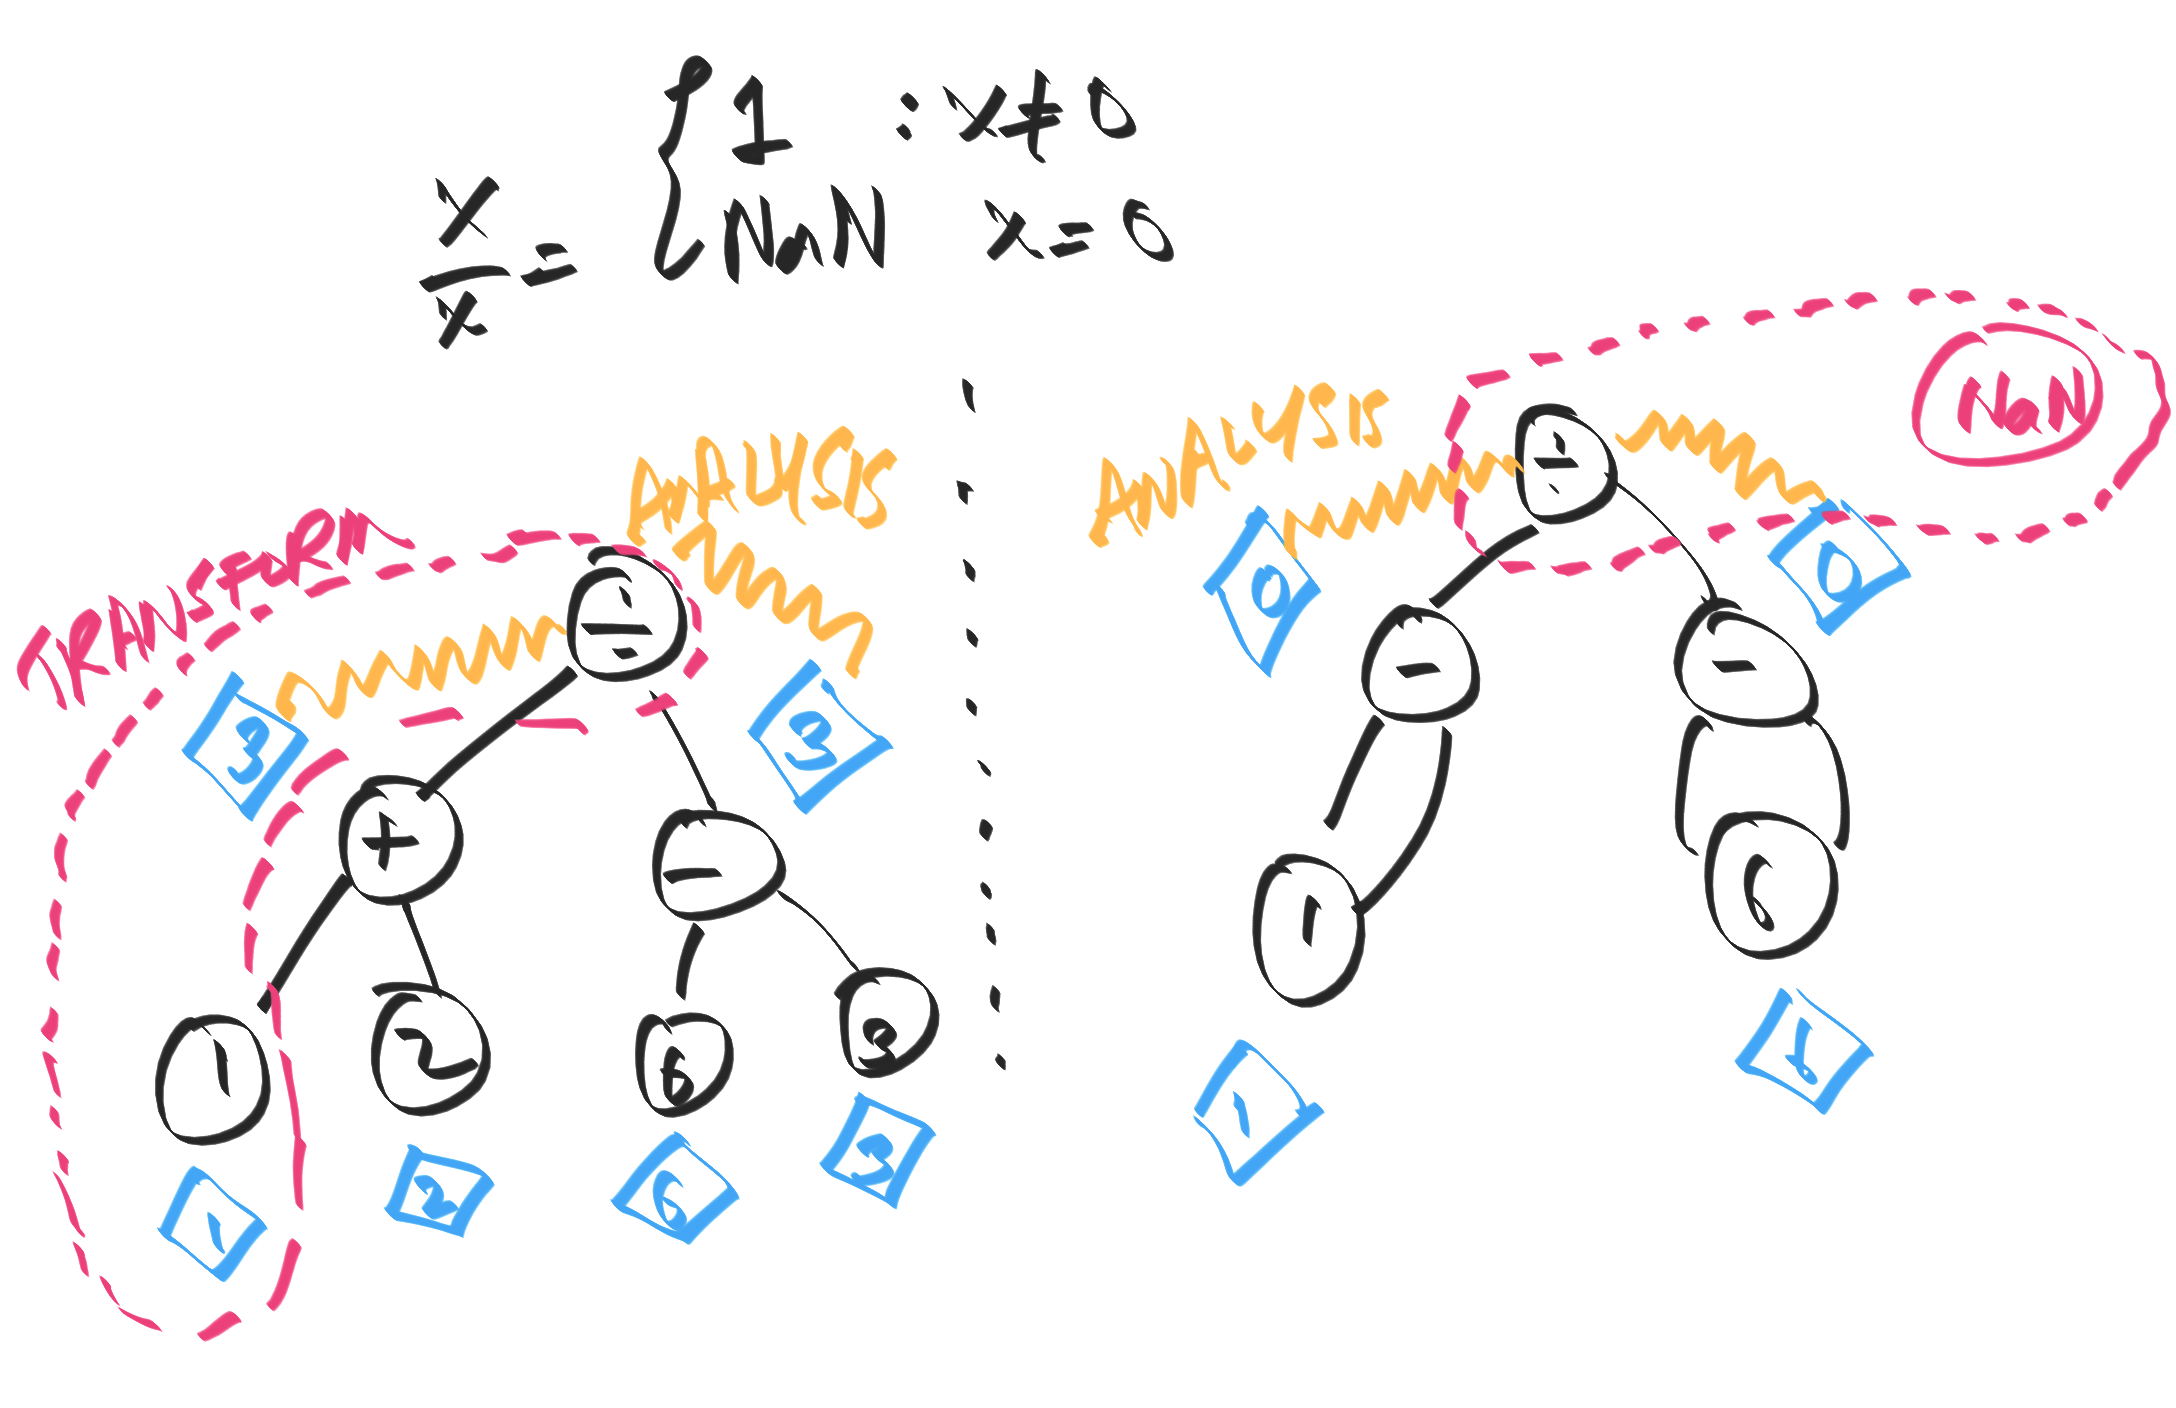
\includegraphics[width=\textwidth]{./rewrite-7.png}
\end{frame}

\begin{frame}[fragile]{Herbie: Using \egg --- Lattice}
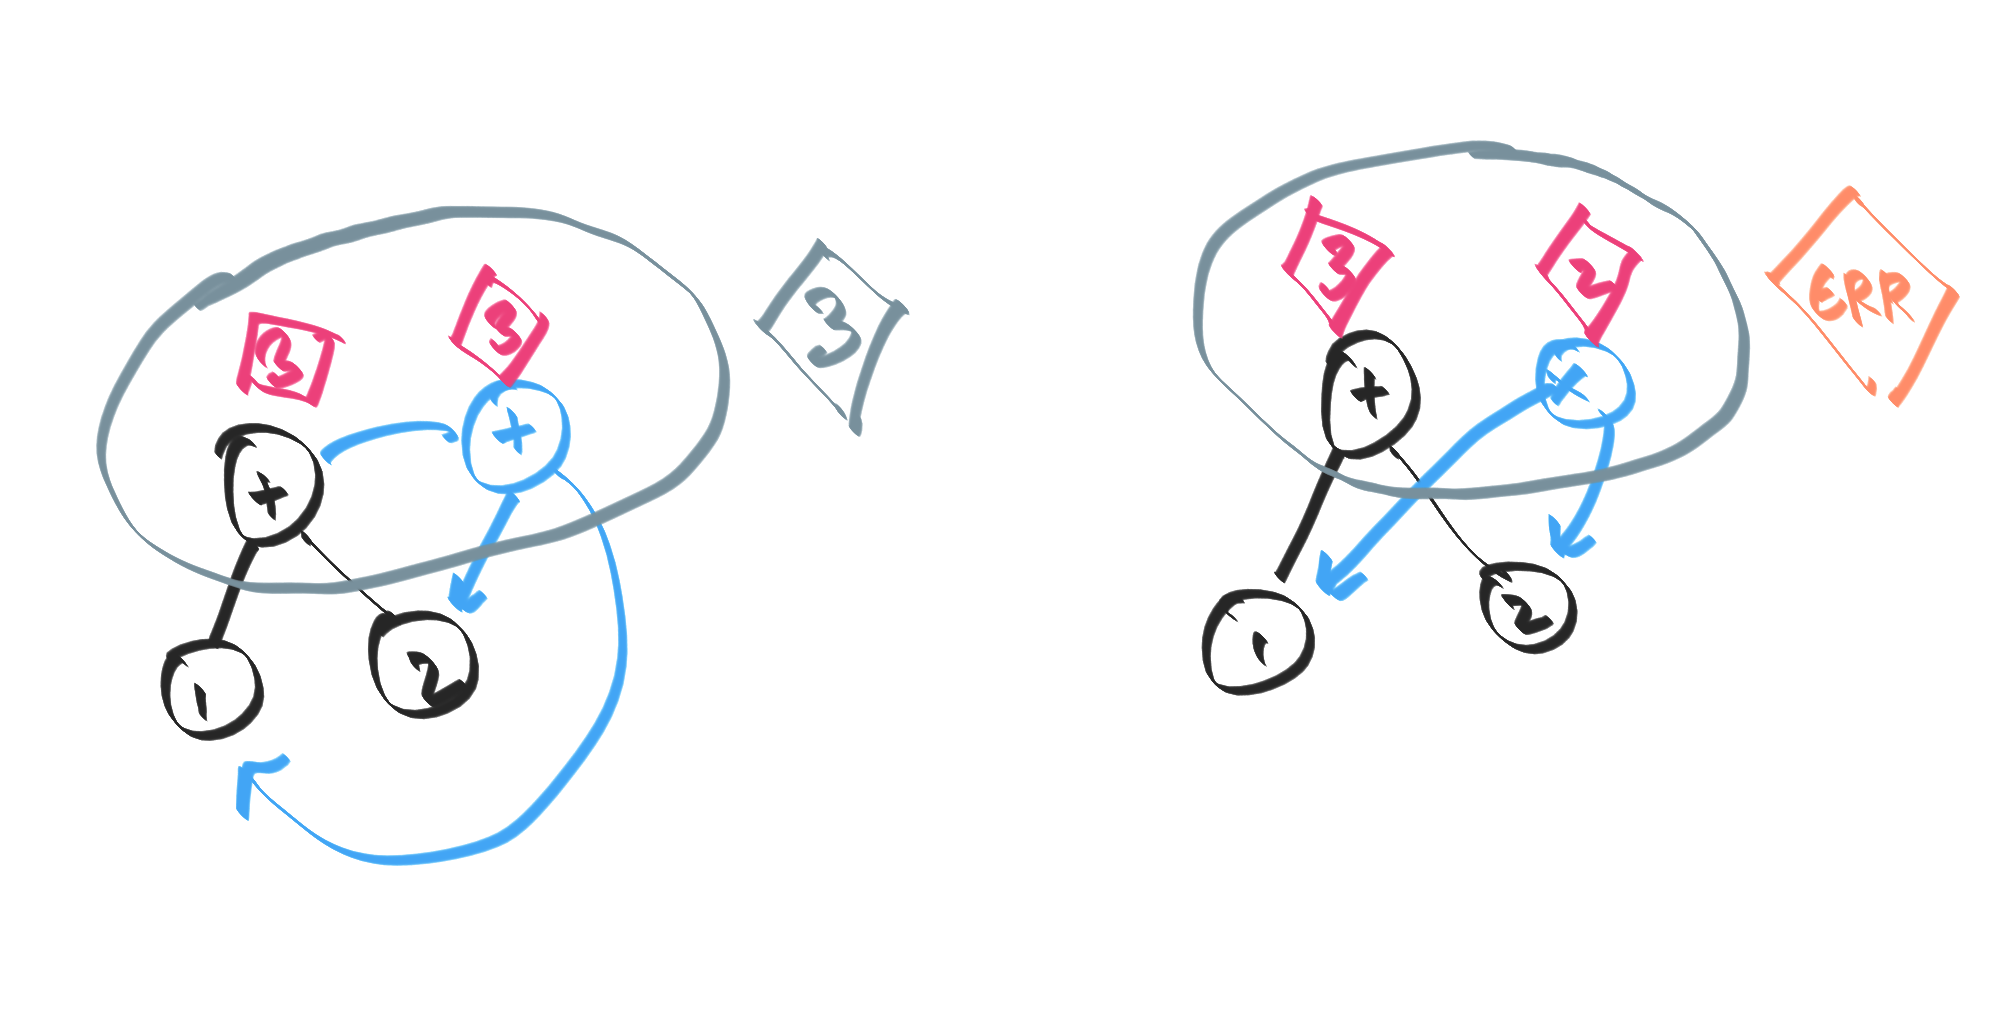
\includegraphics[width=\textwidth]{./analysis-equivalence-classes.png}
\pause
\begin{itemize}
\item Abstract interpretation of equivalence classes.
\item For each node, provide function $\alpha: \node \rightarrow L$ (Abstraction function)
\item $(L, \cap)$ is a join-semilattice.
\item \egg provides for each equivalence class $\class \mapsto \bigcap_{\node \in \class} \alpha(\node) \in L$
\end{itemize}
\end{frame}


\begin{frame}[fragile]{Speedup over prior art: Merging}
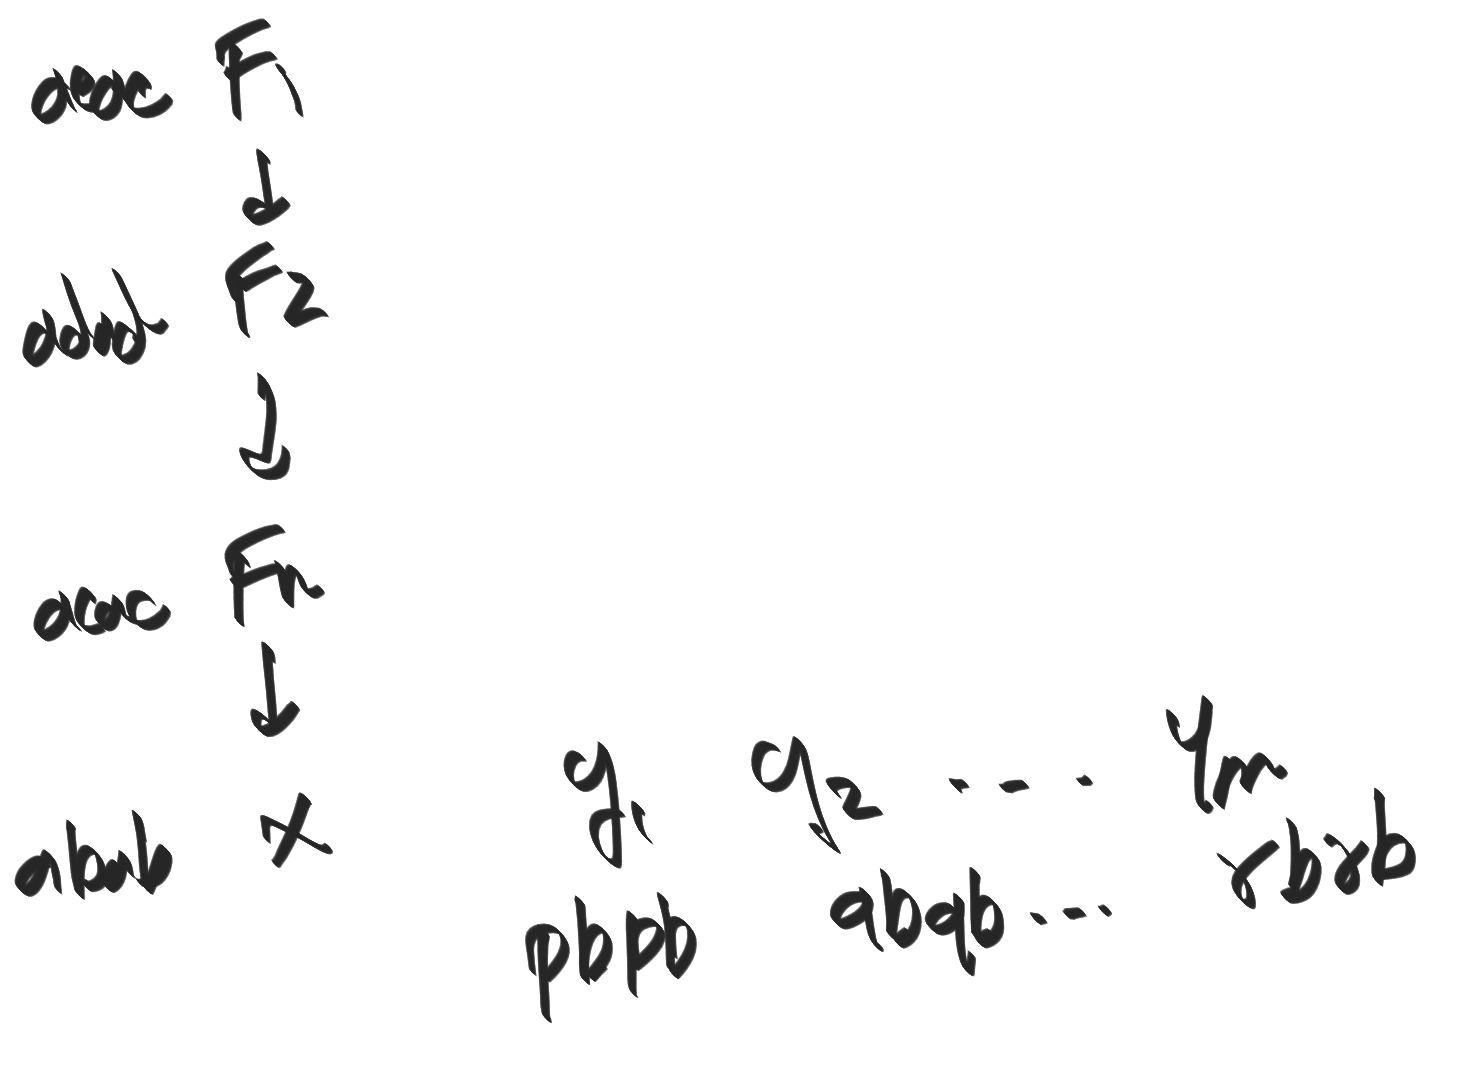
\includegraphics[width=\textwidth]{./eg-2-1.png}
\end{frame}

\begin{frame}[fragile]{Speedup over prior art: Merging}
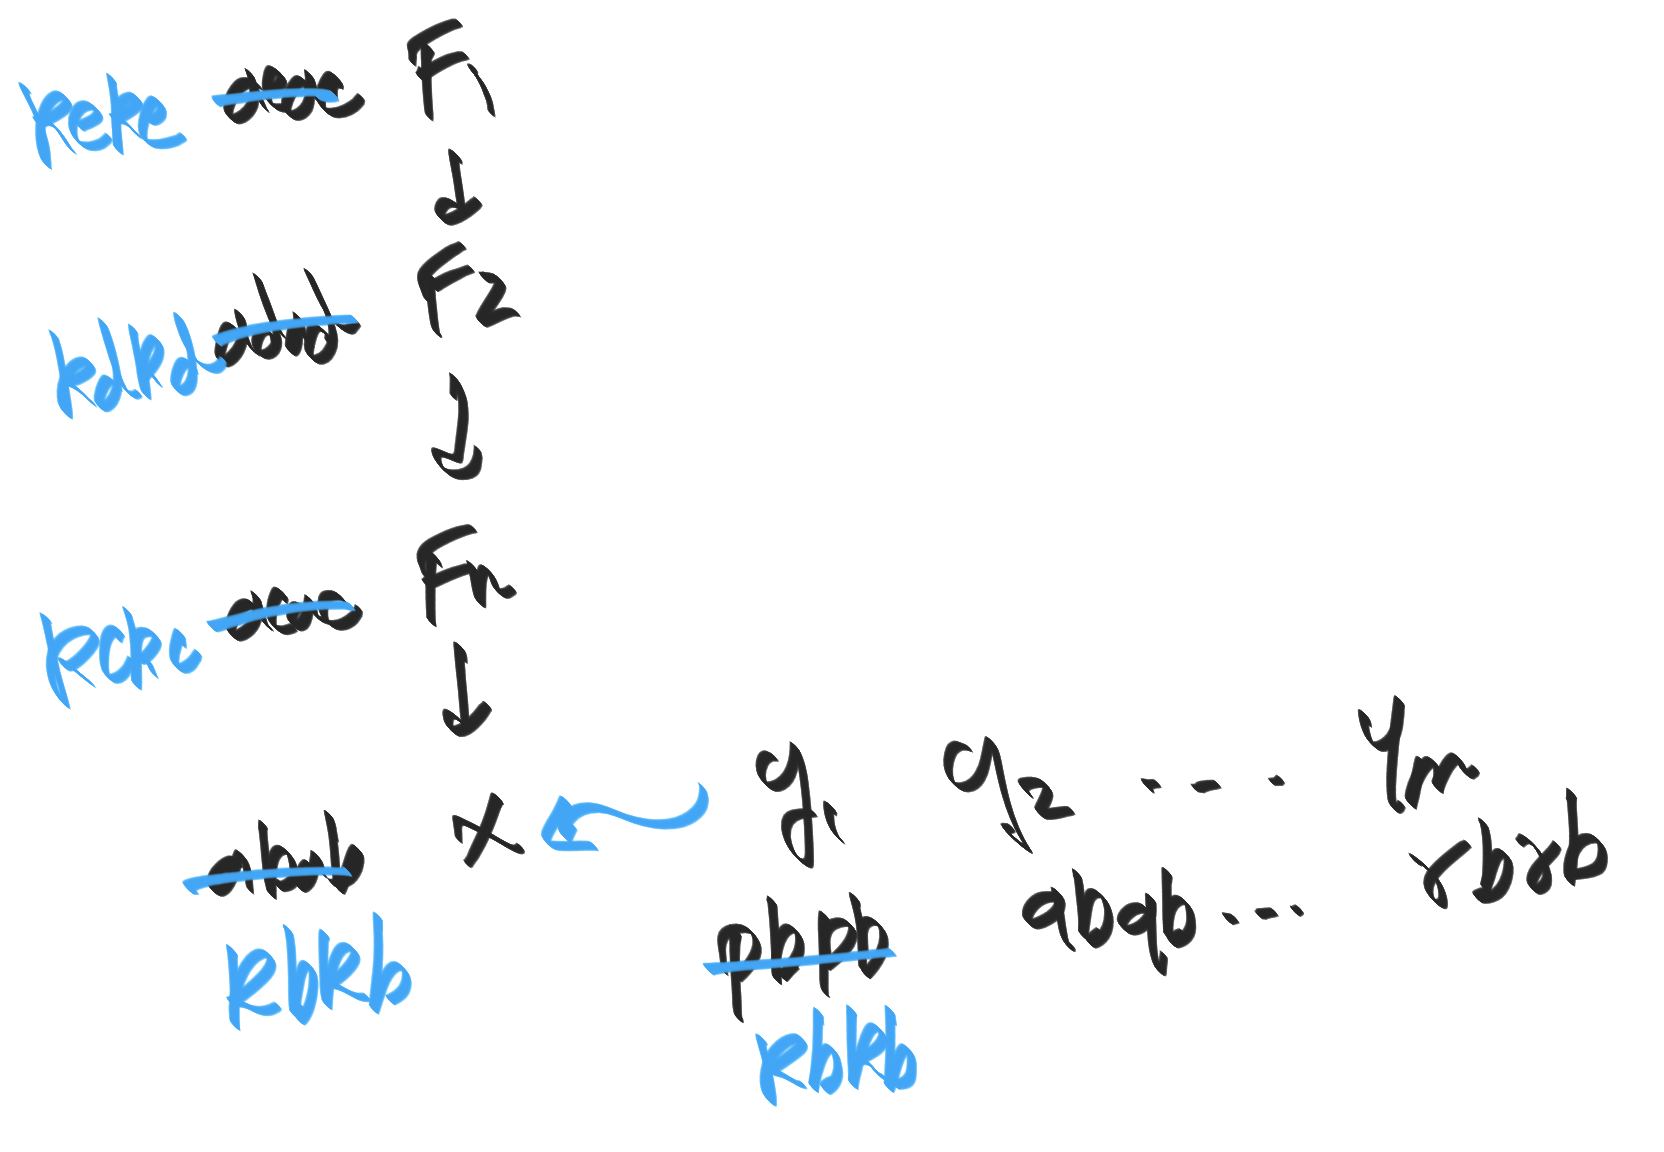
\includegraphics[width=\textwidth]{./eg-2-2.png}
\end{frame}

\begin{frame}[fragile]{Speedup over prior art: Merging}
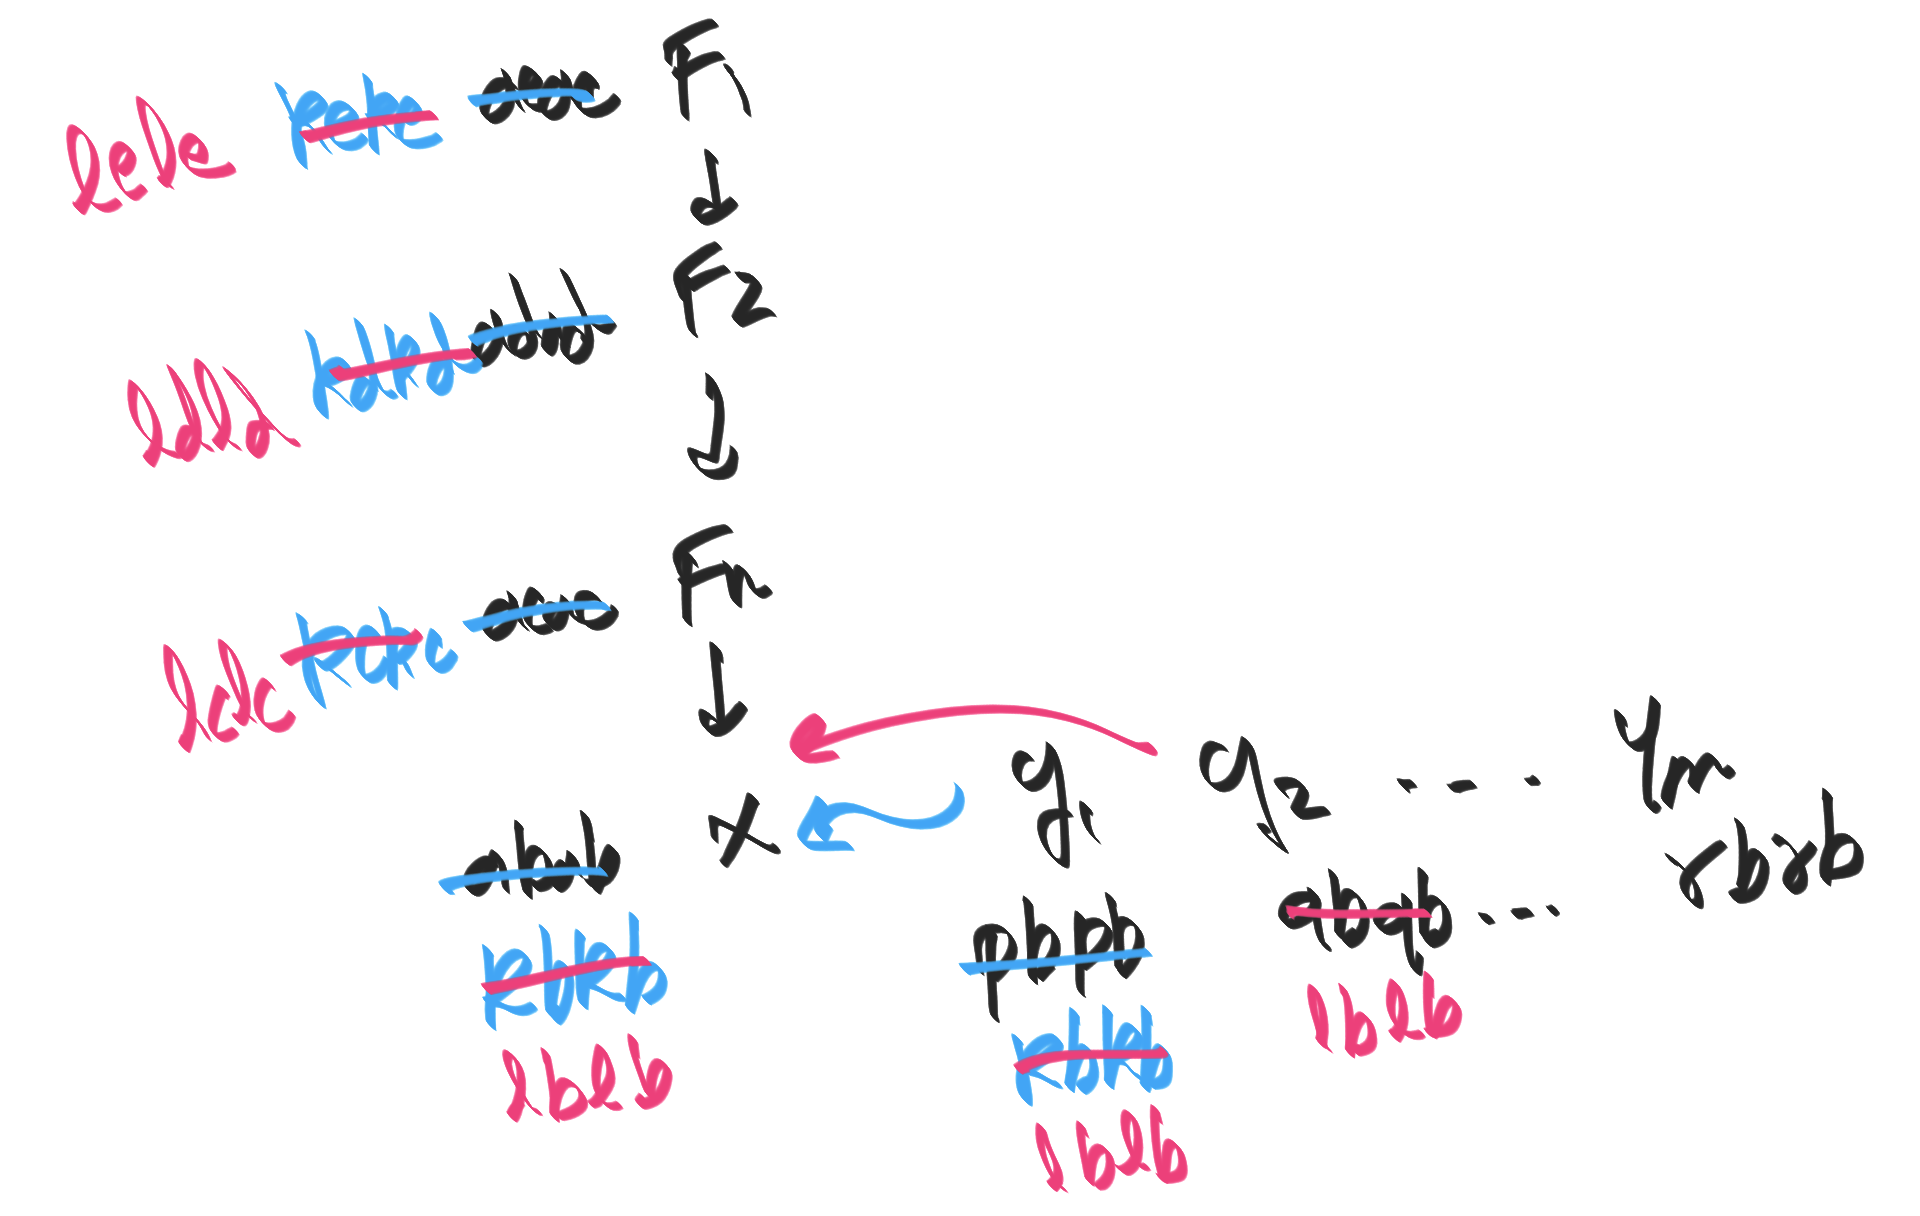
\includegraphics[width=\textwidth]{./eg-2-3.png}
\end{frame}

\begin{frame}[fragile]{Speedup over prior art: Merging}
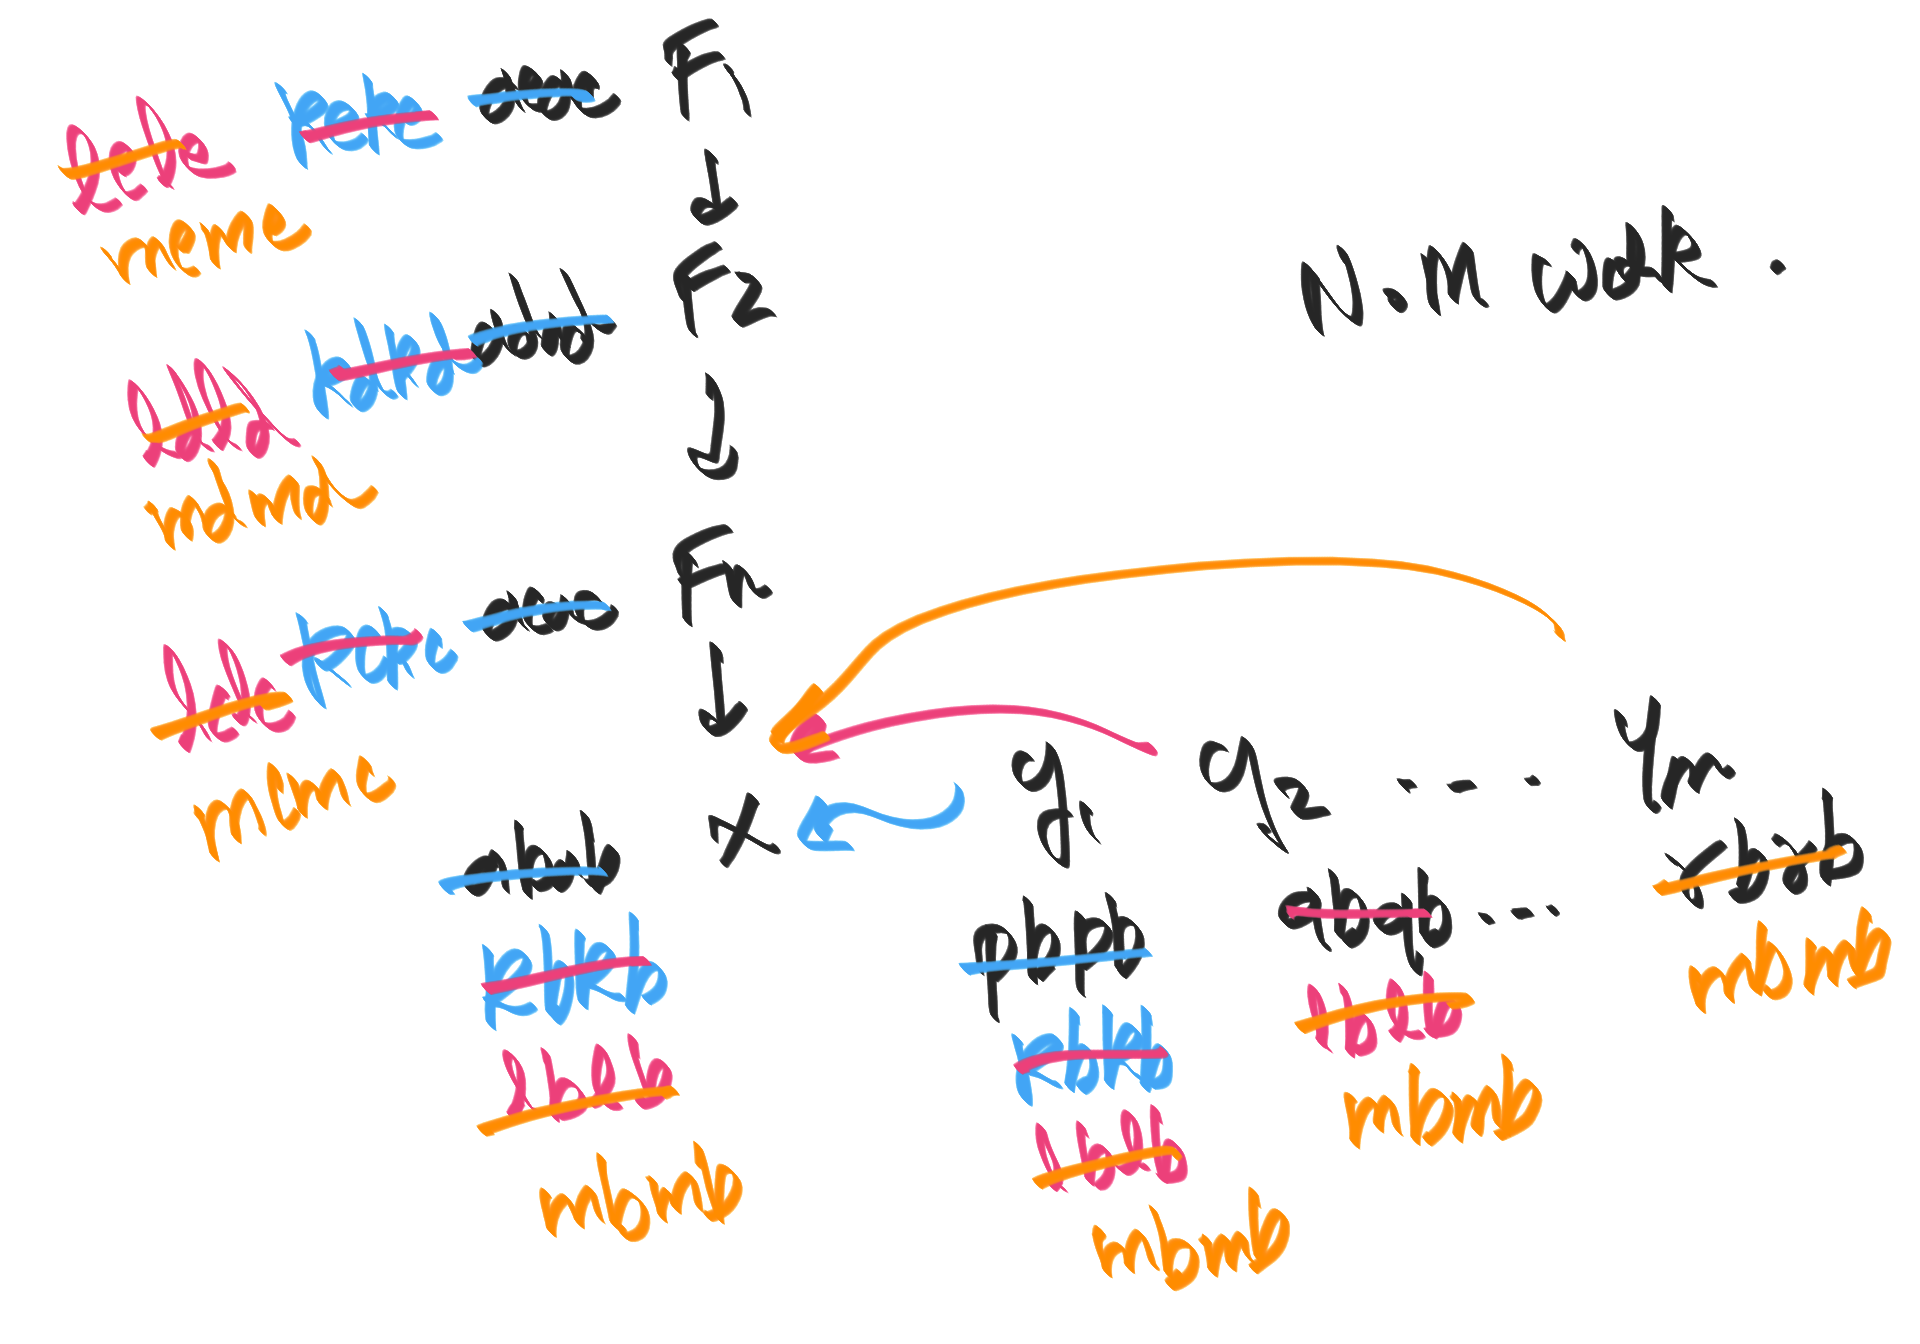
\includegraphics[width=\textwidth]{./eg-2-4.png}
\end{frame}


\begin{frame}[fragile]{Speedup over prior art: Merging}
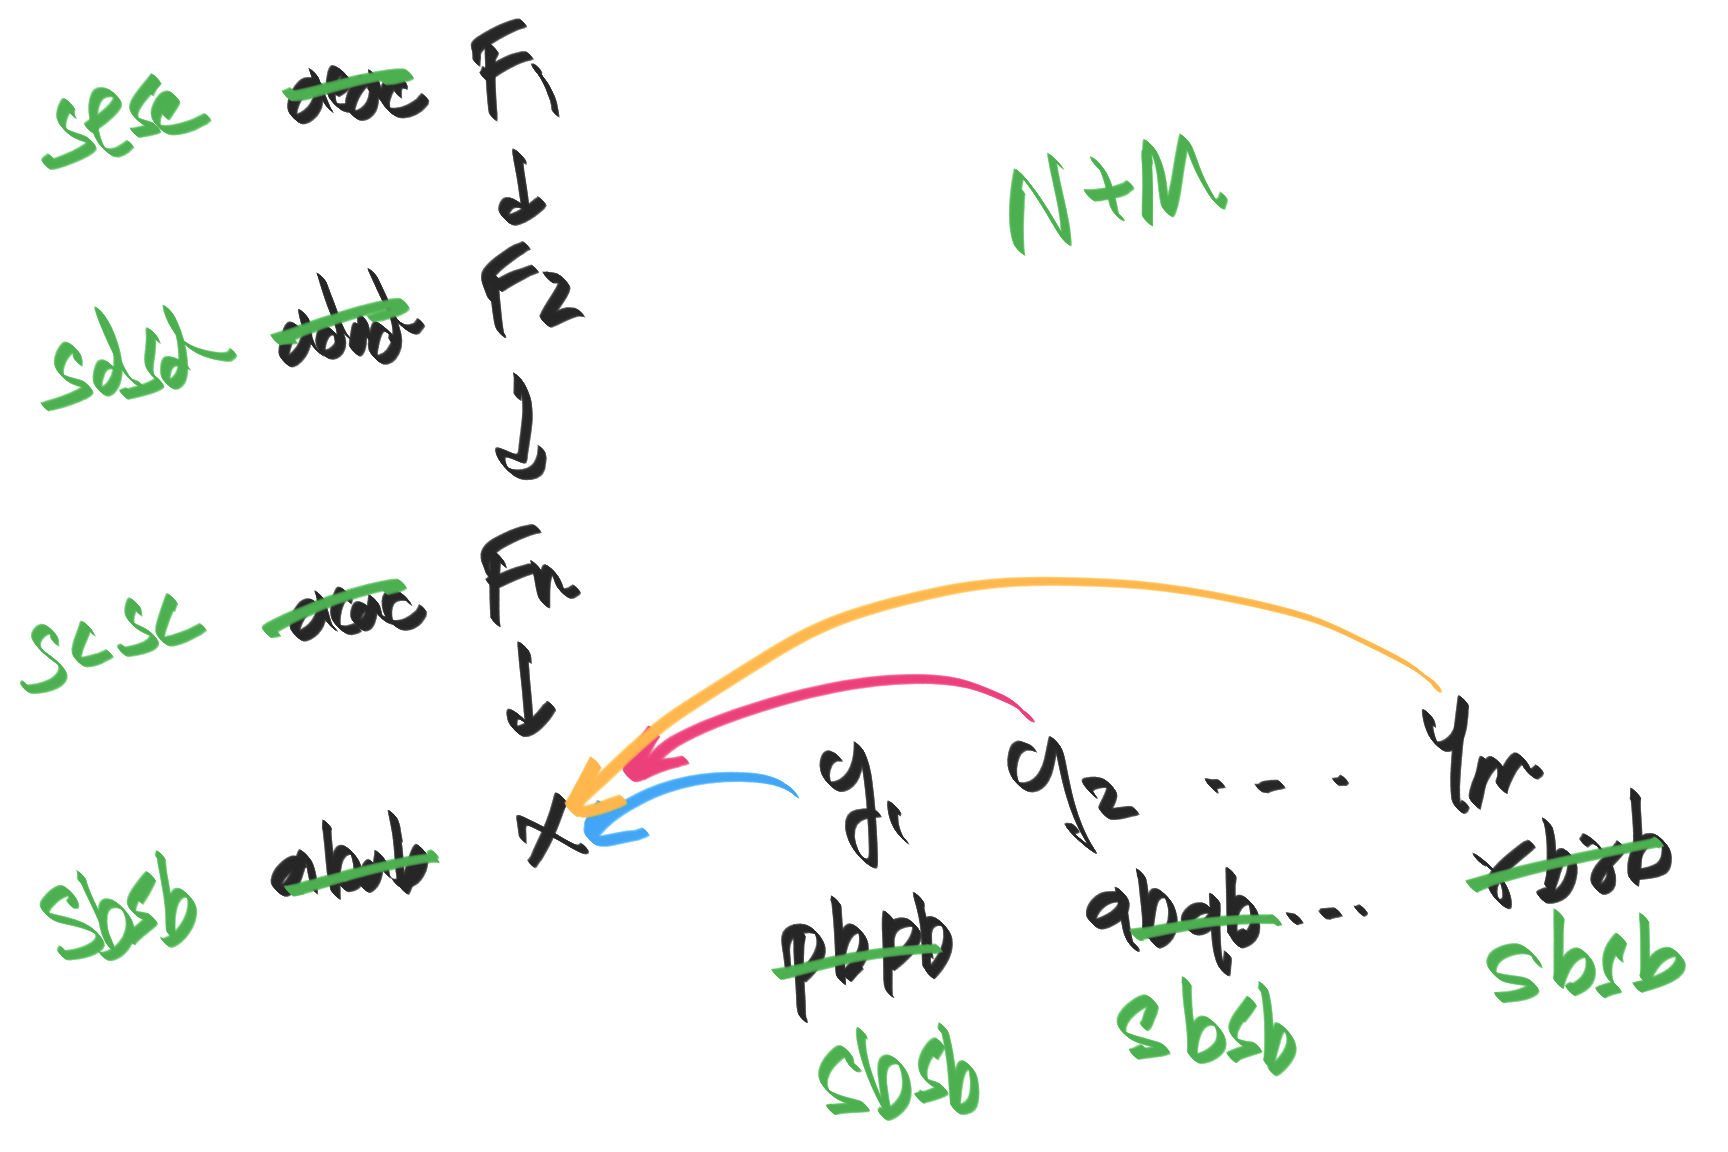
\includegraphics[width=\textwidth]{./eg-2-5.png}
\end{frame}



\begin{frame}[fragile]{Speedup over prior art: Merging}
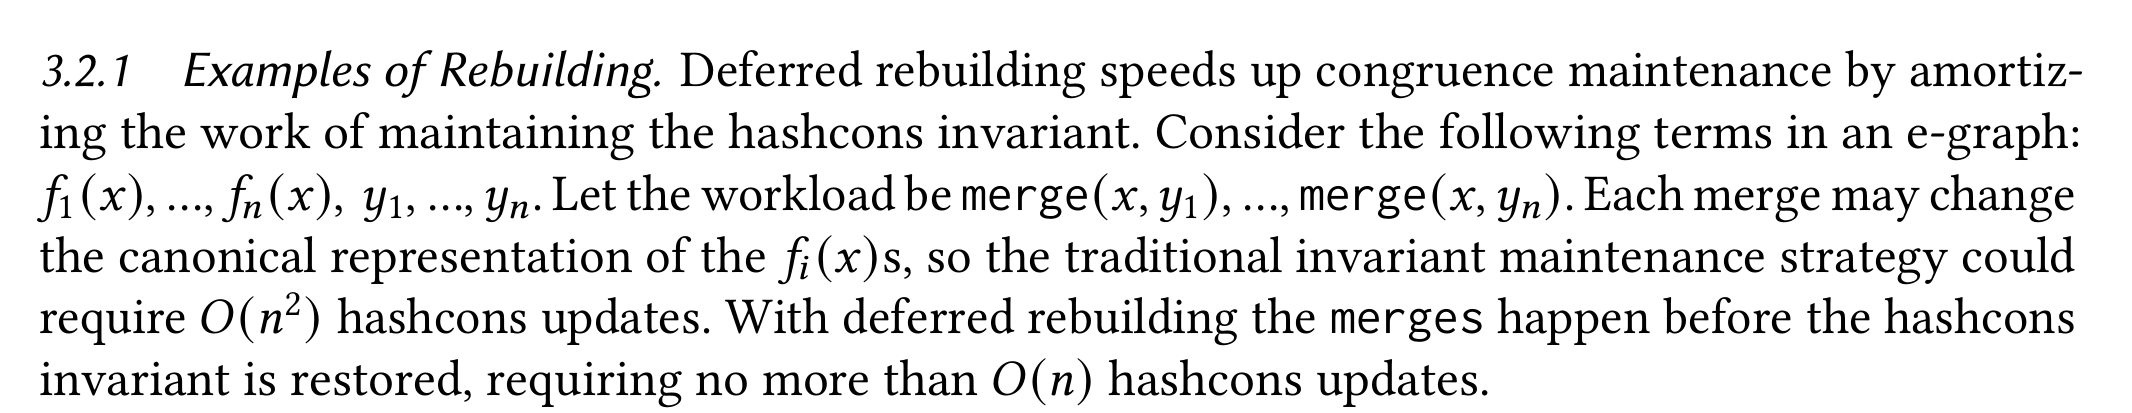
\includegraphics[width=\textwidth]{./eg-2-paper-snippet.png}
\end{frame}



\begin{frame}[fragile]{Lambda calculus in \egg: Dynamic rewrites}
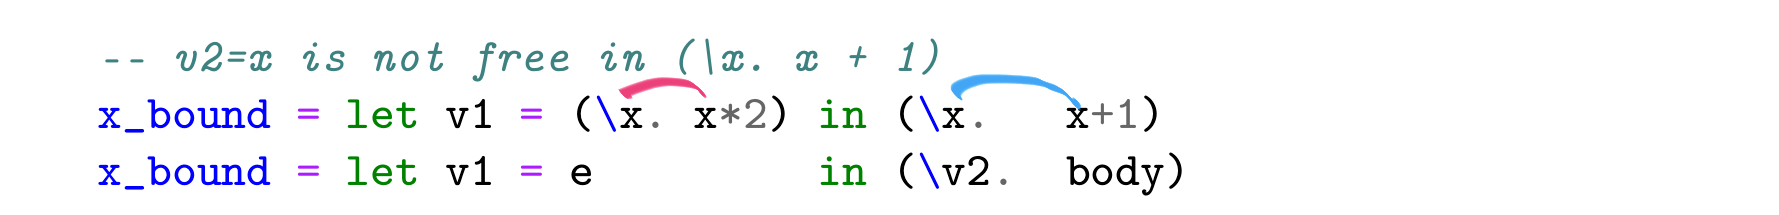
\includegraphics[width=\textwidth]{./lc-1.png}
\pause
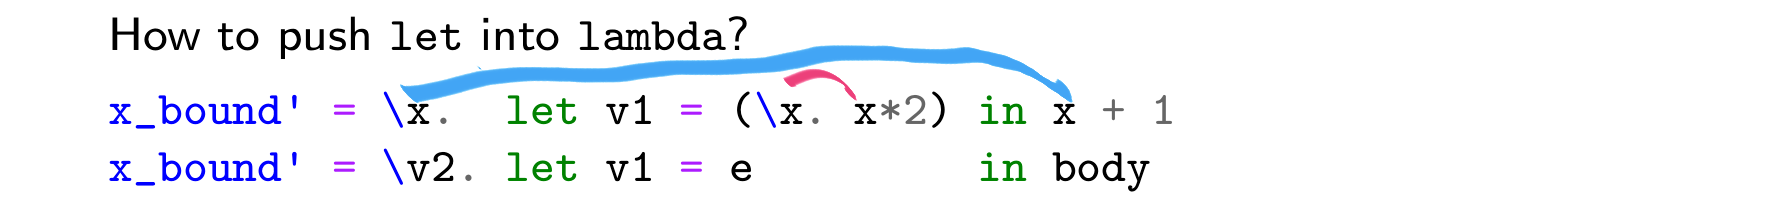
\includegraphics[width=\textwidth]{./lc-2.png}
\pause
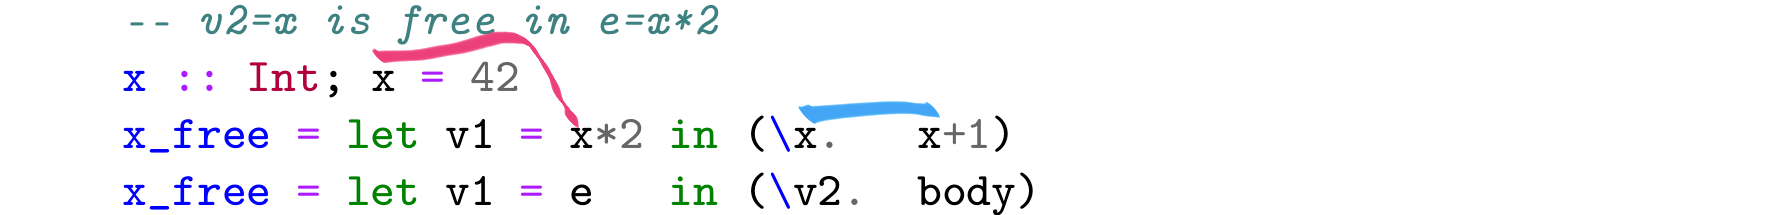
\includegraphics[width=\textwidth]{./lc-3.png}
\pause
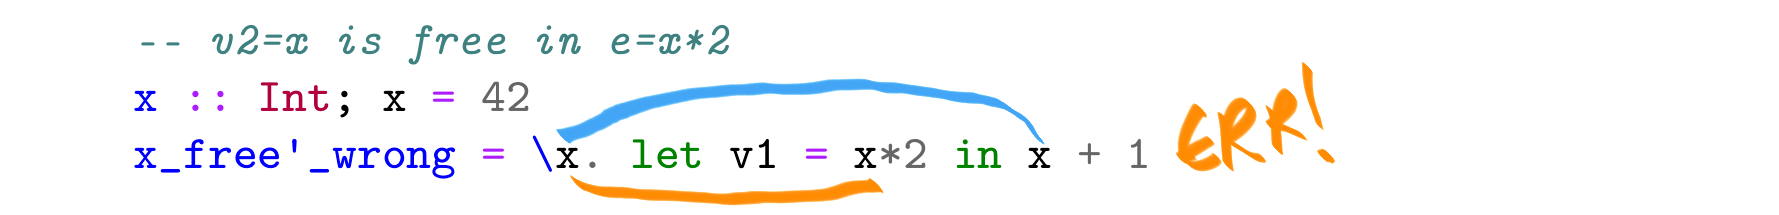
\includegraphics[width=\textwidth]{./lc-4.png}
\pause
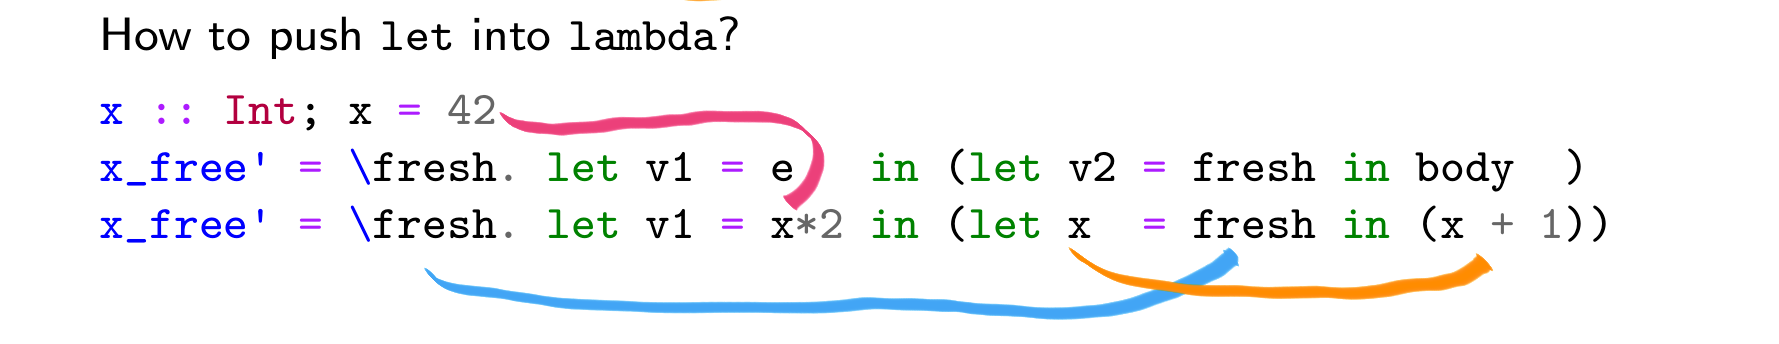
\includegraphics[width=\textwidth]{./lc-5.png}
\end{frame}

% \begin{frame}{Lambda calculus in \egg: constant folding}
% \begin{minted}{rust}
% fn eval(egraph: &EGraph, enode: &Lambda) -> Option<Lambda> {
%     let x = |i: &Id| egraph[*i].data.constant.clone();
%     match enode {
%         Lambda::Num(_) | Lambda::Bool(_) => Some(enode.clone()),
%         Lambda::Add([a, b]) => Some(Lambda::Num(x(a)?.num()? + x(b)?.num()?)),
%         Lambda::Eq([a, b]) => Some(Lambda::Bool(x(a)? == x(b)?)),
%         _ => None,
%     }
% }
% \end{minted}
% \end{frame}

\end{document}
